% !TeX program = lualatex
% Compilación recomendada: latexmk -lualatex tesis.tex
\RequirePackage{fix-cm}
\documentclass[11pt,a4paper,oneside]{report}

\usepackage{fontspec}
\setmainfont{Arial}
\setsansfont{Arial}
% La guía muestra Poppins para la línea institucional. En este entorno no está
% instalada; se usa la alternativa sans serif disponible (Arial).
\newcommand{\poppins}{\sffamily}
\usepackage[spanish,es-nodecimaldot,es-noshorthands]{babel}
\usepackage{csquotes}
\usepackage{geometry}
\geometry{left=3cm,top=3cm,right=2.5cm,bottom=2.5cm,headheight=14pt,headsep=0.6cm}
\usepackage{setspace}
\onehalfspacing
\usepackage{microtype}
\usepackage{graphicx}
\graphicspath{{imagenes/}}
\usepackage{booktabs,longtable,tabularx,array,multirow,makecell,threeparttable}
\usepackage{pdflscape}
\usepackage{ragged2e}
\usepackage{enumitem}
\usepackage{etoolbox}
\usepackage{titlesec}
\usepackage{fancyhdr}
\usepackage{amsmath,amssymb,mathtools}
\usepackage{siunitx}
\sisetup{output-decimal-marker={,},per-mode=symbol}
\usepackage{xcolor,colortbl}
\definecolor{unired}{HTML}{8B1A1A}
\definecolor{darkblue}{HTML}{17365D}
\definecolor{lightblue}{HTML}{DCE6F1}
\definecolor{lightgray}{HTML}{F2F2F2}
\usepackage{tikz}
\usetikzlibrary{arrows.meta,positioning,shapes.geometric,fit,calc}
\usepackage{newfloat}
\usepackage{float}
\DeclareFloatingEnvironment[fileext=loe,listname={Listado de fórmulas},name=Fórmula,placement=htbp]{formula}
\usepackage{caption}
\captionsetup{font=small,labelfont=bf,justification=centering}
\captionsetup[table]{font=footnotesize}
\AtBeginEnvironment{table}{\footnotesize}
\usepackage[hidelinks]{hyperref}
\hypersetup{
  pdftitle={DISEÑO Y EVALUACIÓN DE UNA RED NEURONAL INFORMADA POR FÍSICA PARA ESTIMAR LA TEMPERATURA Y LA AMPACIDAD DE CABLES ELÉCTRICOS ENTERRADOS EN ENTORNOS HETEROGÉNEOS},
  pdfauthor={Luis Enrique Koc Góngora y Herbert Antonio Meléndez García},
  pdfsubject={Tesis de Maestría en Inteligencia Artificial, FIIS-UNI}
}
\usepackage{bookmark}
\usepackage[backend=biber,style=apa,sortcites=true,sorting=nyt,maxcitenames=2,maxbibnames=20]{biblatex}
\DeclareLanguageMapping{spanish}{spanish-apa}
\DeclareFieldFormat{postnote}{#1}
\DeclareDelimFormat{postnotedelim}{\addcolon}
\addbibresource{referencias.bib}
\addbibresource{../Benchmarks/references_selection.bib}

\setcounter{tocdepth}{4}
\setcounter{secnumdepth}{4}
\setlength{\parindent}{0pt}
\setlength{\parskip}{12pt}
\setlength{\emergencystretch}{3em}
\setlist{leftmargin=1.1cm,topsep=.5\baselineskip,itemsep=.5\baselineskip,parsep=0pt,partopsep=0pt}
\renewcommand{\arraystretch}{1.18}
\newcolumntype{Y}{>{\RaggedRight\arraybackslash}X}
\newcolumntype{J}{>{\justifying\arraybackslash}X}
\newcolumntype{L}[1]{>{\RaggedRight\arraybackslash}p{#1}}
\newcolumntype{C}[1]{>{\Centering\arraybackslash}p{#1}}

% La Guía UNI prescribe Arial 11 para el cuerpo y hasta cuatro niveles.
\titleformat{\chapter}[hang]
  {\normalfont\bfseries\fontsize{11}{13.2}\selectfont}
  {\MakeUppercase{\chaptername}\ \thechapter.}{0.75em}{\MakeUppercase}
\titleformat{name=\chapter,numberless}[block]
  {\normalfont\bfseries\fontsize{11}{13.2}\selectfont}
  {}{0pt}{\MakeUppercase}
\titlespacing*{\chapter}{0pt}{0pt}{0.75\baselineskip}
\titleformat{\section}
  {\normalfont\bfseries\fontsize{11}{13.2}\selectfont}
  {\thesection}{0.75em}{\MakeUppercase}
\titlespacing*{\section}{0pt}{1.0\baselineskip}{0.25\baselineskip}
\titleformat{\subsection}
  {\normalfont\bfseries\fontsize{11}{13.2}\selectfont}
  {\thesubsection}{0.75em}{\MakeUppercase}
\titlespacing*{\subsection}{0pt}{0.75\baselineskip}{0.25\baselineskip}
\titleformat{\subsubsection}
  {\normalfont\bfseries\fontsize{11}{13.2}\selectfont}
  {\thesubsubsection}{0.75em}{\MakeUppercase}
\titlespacing*{\subsubsection}{0pt}{0.5\baselineskip}{0.25\baselineskip}
\renewcommand\theparagraph{\alph{paragraph})}
\titleformat{\paragraph}
  {\normalfont\bfseries\fontsize{11}{13.2}\selectfont}
  {\theparagraph}{0.75em}{}
\titlespacing*{\paragraph}{0pt}{0.35\baselineskip}{0.2\baselineskip}

\fancypagestyle{tesis}{
  \fancyhf{}
  \fancyhead[R]{\normalfont\fontsize{11}{13.2}\selectfont\thepage}
  \renewcommand{\headrulewidth}{0pt}
  \renewcommand{\footrulewidth}{0pt}
}
\fancypagestyle{plain}{
  \fancyhf{}
  \fancyhead[R]{\normalfont\fontsize{11}{13.2}\selectfont\thepage}
  \renewcommand{\headrulewidth}{0pt}
  \renewcommand{\footrulewidth}{0pt}
}
\pagestyle{tesis}

\addto\captionsspanish{%
  \renewcommand{\contentsname}{Índice de contenidos}%
  \renewcommand{\listfigurename}{Lista de figuras}%
  \renewcommand{\listtablename}{Lista de tablas}%
  \renewcommand{\tablename}{Tabla}%
}

\newcommand{\Tmax}{T_{\max}}
\newcommand{\Imax}{I_{\max}}
\newcommand{\kx}{k(x,y)}
\newcommand{\rhoth}{\rho_{\mathrm{th}}}
\newcommand{\pct}{\mbox{\char37}}
\newcommand{\tituloTesis}{DISEÑO Y EVALUACIÓN DE UNA RED NEURONAL INFORMADA POR FÍSICA PARA ESTIMAR LA TEMPERATURA Y LA AMPACIDAD DE CABLES ELÉCTRICOS ENTERRADOS EN ENTORNOS HETEROGÉNEOS}

% Marca institucionalmente visible para contenidos aún no sustentados por evidencia.
\newcommand{\pendiente}[1]{%
  \par\medskip
  \begin{center}
    {\color{red}\bfseries\fontsize{18}{22}\selectfont PENDIENTE}
  \end{center}
  {\color{red}\itshape #1\par}
  \medskip
}

\begin{document}
\hypersetup{pageanchor=false}

\begin{titlepage}
\thispagestyle{empty}
\begin{singlespace}
\setlength{\parskip}{0pt}
\begin{center}
{\poppins\bfseries\fontsize{22}{26}\selectfont UNIVERSIDAD NACIONAL DE INGENIERÍA\par}
\vspace{0.35cm}
{\bfseries\fontsize{16}{19}\selectfont UNIDAD DE POSGRADO DE LA FACULTAD DE INGENIERÍA INDUSTRIAL Y DE SISTEMAS\par}
{\bfseries\fontsize{16}{19}\selectfont ESCUELA DE POSGRADO\par}
\vspace{0.35cm}

\includegraphics[width=6.7cm]{logo_UNI.png}
\vspace{0.25cm}

{\bfseries\fontsize{14}{17}\selectfont TESIS\par}
\vspace{0.25cm}
{\bfseries\fontsize{12}{14.4}\selectfont\MakeUppercase{\tituloTesis}\par}

\vfill
{\fontsize{12}{14.4}\selectfont
PARA OBTENER EL GRADO ACADÉMICO DE\par
MAESTRO CON MENCIÓN EN:\par
INTELIGENCIA ARTIFICIAL\par}

\vspace{0.55cm}
{\bfseries\fontsize{12}{14.4}\selectfont ELABORADA POR:\par}
{\bfseries\fontsize{12}{14.4}\selectfont LUIS ENRIQUE KOC GÓNGORA\par}
{\bfseries\fontsize{12}{14.4}\selectfont HERBERT ANTONIO MELÉNDEZ GARCÍA\par}

\vspace{0.5cm}
{\bfseries\fontsize{12}{14.4}\selectfont ASESOR: SAMUEL OPORTO\par}

\vfill
{\bfseries\fontsize{14}{17}\selectfont LIMA, PERÚ\par}
{\bfseries\fontsize{12}{14.4}\selectfont 2026\par}
\end{center}
\end{singlespace}
\end{titlepage}

\hypersetup{pageanchor=true}
\pagenumbering{roman}
\setcounter{page}{2}

\chapter*{DATOS GENERALES}
\addcontentsline{toc}{chapter}{DATOS GENERALES}
\begin{tabularx}{\textwidth}{>{\bfseries\RaggedRight\arraybackslash}p{4.1cm}J}
\toprule
\rowcolor{lightgray}
Elemento & Descripción \\
\midrule
Título & \tituloTesis. \\
Tesistas & Luis Enrique Koc Góngora; Herbert Antonio Meléndez García. \\
Programa & Maestría en Inteligencia Artificial. \\
Unidad académica & Unidad de Posgrado de la Facultad de Ingeniería Industrial y de Sistemas, Universidad Nacional de Ingeniería. \\
Tipo de tesis & Maestría de especialización o profesionalizante. \\
Objeto de estudio & Arreglo de cables eléctricos enterrados y su entorno térmico. \\
Artefacto & Modelo y prototipo computacional 2D basado en redes neuronales informadas por física. \\
Lugar de desarrollo & Entorno computacional de la FIIS-UNI y casos de referencia documentados. \\
\bottomrule
\end{tabularx}

\chapter*{DEDICATORIA}
\addcontentsline{toc}{chapter}{DEDICATORIA}

\pendiente{Incorporar el texto personal aprobado por ambos tesistas. Esta sección no puede derivarse del plan de tesis.}


\chapter*{AGRADECIMIENTOS}
\addcontentsline{toc}{chapter}{AGRADECIMIENTOS}

\pendiente{Redactar los agradecimientos institucionales y personales después de confirmar nombres, cargos y contribuciones.}


\chapter*{COPIA DE DOCUMENTOS}
\addcontentsline{toc}{chapter}{COPIA DE DOCUMENTOS}

\pendiente{Insertar los documentos exigidos por la Escuela de Posgrado: nombramiento o aprobación, acta de sustentación, certificado de idioma, declaración de autenticidad y demás constancias aplicables.}



\begingroup
\singlespacing
\tableofcontents
\listoffigures
\listoftables
\listofformulas
\endgroup

\chapter*{RESUMEN}
\addcontentsline{toc}{chapter}{RESUMEN}

La ampacidad de un cable eléctrico enterrado depende de las pérdidas internas y de la capacidad del entorno para evacuar calor. La humedad, los estratos, el lecho de asiento y el suelo de relleno producen una conductividad térmica espacialmente variable que puede modificar el campo de temperatura, la temperatura máxima del conductor y la corriente admisible. Esta investigación diseña y evalúa un artefacto computacional bidimensional basado en una red neuronal informada por física. El artefacto incorpora la ecuación estacionaria de conducción, las condiciones de contorno e interfaz y la conductividad espacial dentro del entrenamiento. La ciencia del diseño organiza la especificación, construcción, demostración, evaluación y comunicación del artefacto. La verificación considera soluciones analíticas o manufacturadas, referencias FEM convergentes y casos publicados; además, registra exactitud térmica, consistencia física, robustez y reproducibilidad.

\pendiente{Completar el resumen con los resultados cuantitativos principales, la conclusión central y el impacto estimado. Ajustar la extensión y las palabras clave después de cerrar el Capítulo III.}

\noindent\textbf{Palabras clave:} cable subterráneo; ampacidad; heterogeneidad térmica; conductividad del suelo; red neuronal informada por física; ciencia del diseño.

\chapter*{ABSTRACT}
\addcontentsline{toc}{chapter}{ABSTRACT}

The ampacity of an underground power cable depends on internal losses and on the ability of the surrounding environment to dissipate heat. Moisture, soil layers, bedding, and backfill create a spatially varying thermal conductivity that may alter the temperature field, the maximum conductor temperature, and the allowable current. This research designs and evaluates a two-dimensional computational artifact based on a physics-informed neural network. The artifact embeds the steady-state heat equation, boundary and interface conditions, and spatial conductivity into training. Design science organizes the specification, construction, demonstration, evaluation, and communication of the artifact. Verification uses analytical or manufactured solutions, converged FEM references, and published cases, while recording thermal accuracy, physical consistency, robustness, and reproducibility.

\pendiente{Traducir la versión final del resumen después de incorporar resultados, conclusión e impacto. Verificar que ambas versiones sean equivalentes.}

\noindent\textbf{Keywords:} underground cable; ampacity; thermal heterogeneity; soil thermal conductivity; physics-informed neural network; design science research.


\chapter*{INTRODUCCIÓN}
\addcontentsline{toc}{chapter}{INTRODUCCIÓN}

En el Perú, la máxima demanda del Sistema Eléctrico Interconectado Nacional aumentó de \SI{4579}{\mega\watt} en 2010 a \SI{7942}{\mega\watt} en 2025. En el mismo período, la participación conjunta de la generación solar y eólica pasó de un valor cercano a cero a 9,5\,\pct{}. Estos cambios aumentan la exigencia de transportar energía y aprovechar la capacidad disponible de la red \parencites{minem2025anuario2024}{minem2025indicadoresDiciembre}{coesMaximaDemanda}{iea2025transmissiongrid}.

Los cables enterrados se usan en redes colectoras de plantas solares y eólicas y en tramos donde el espacio, la servidumbre, la seguridad o la integración urbana dificultan construir líneas aéreas \parencite{cigre2023overheadLines}. Su capacidad de transporte depende de la evacuación del calor hacia el lecho de asiento, el suelo de relleno y el suelo nativo. La ampacidad $\Imax$ es la corriente que un cable puede transportar de manera sostenida, bajo condiciones especificadas, sin que la temperatura máxima del conductor $\Tmax$ supere el límite térmico admisible \parencites[cláusulas~4--5]{iec60287}[3--5]{enescu2020}.

El objeto de estudio es el arreglo de cables--entorno térmico, formado por los cables, su disposición y los materiales circundantes. El entorno es heterogéneo cuando su conductividad térmica $\kx$ varía por humedad, estratos o interfaces. Esa variación cambia el campo $T(x,y)$, del cual se obtienen $\Tmax$ y $\Imax$ \parencites[3--4]{enescu2021}[1,6--7]{khumalo2025}[3]{xing2023}.

El problema aparece cuando una propiedad homogénea equivalente sustituye esa distribución espacial. La simplificación puede ocultar zonas de baja disipación o producir estimaciones conservadoras. Los métodos de campo, como FEM, pueden representar la geometría y los materiales con detalle, pero requieren construir, mallar y verificar cada escenario \parencites[41--42,93--99]{cigre2025}[1--3,12]{aldulaimi2024}.

La investigación propone un artefacto basado en una red neuronal informada por física (PINN) que incorpora la ecuación de conducción de calor y sus condiciones de frontera e interfaz. El artefacto aproxima $T(x,y)$, estima $\Tmax$ e $\Imax$ y conserva registros de verificación. La ciencia del diseño organiza la relación entre problema práctico, construcción tecnológica y evidencia de evaluación \parencites[54--56]{peffers2007}[342--350]{gregor2013}.

El Capítulo I delimita el problema, los objetivos y la metodología. El Capítulo II desarrolla los antecedentes y las bases teóricas. El Capítulo III presenta la solución y reserva la evidencia de desarrollo, resultados, discusión e impacto. El Capítulo IV se destina a las conclusiones y recomendaciones que podrán formularse después de evaluar el artefacto.



\clearpage
\pagenumbering{arabic}

\chapter{PLANTEAMIENTO DEL PROBLEMA}
\label{ch:planteamiento}

Este capítulo delimita la dificultad práctica que origina el estudio y la convierte en un problema abordable mediante una solución tecnológica. Además, establece los objetivos y el diseño metodológico que conectan la heterogeneidad térmica con la construcción y evaluación del artefacto PINN.

\section{DIAGNÓSTICO}
\label{sec:diagnostico}

Las redes eléctricas deben atender el crecimiento de la demanda e integrar centrales de generación ubicadas en distintos puntos del sistema. En el Perú, la producción eléctrica aumentó de \SI{35908}{\giga\watt\hour} en 2010 a \SI{65109}{\giga\watt\hour} en 2025, según la serie histórica y el cierre preliminar consultados \parencites[sec.~10.4]{minem2025anuario2024}[cuadro~4]{minem2025indicadoresDiciembre}.

La composición de la generación también cambió. La participación conjunta de las fuentes solar y eólica alcanzó 9,5\,\pct{} de la producción nacional en 2025 \parencite[cuadro~4]{minem2025indicadoresDiciembre}. La expansión de estas fuentes requiere redes colectoras, conexiones y capacidad de transporte entre nuevos puntos del SEIN \parencites{coes2023diagnostico2025_2034}{iea2025transmissiongrid}.

Los cables enterrados intervienen en redes colectoras y en enlaces donde existen restricciones de espacio, servidumbre, seguridad o integración urbana \parencite{cigre2023overheadLines}. En estas instalaciones, la capacidad no depende solo de la sección del conductor. También depende del camino térmico formado por las capas del cable, el lecho de asiento, el suelo de relleno y el suelo nativo \parencites{enescu2020}{enescu2021}.

Los métodos normativos relacionan pérdidas, resistencias térmicas y temperatura para calcular la corriente admisible \parencites{neher1957}{iec60287}{iec60853}. Sin embargo, suelen representar el entorno mediante propiedades equivalentes. La humedad, el secado, los estratos y los materiales de relleno pueden generar regiones con distinta conductividad y alterar el camino local del calor \parencites[4--6]{enescu2021}[1--3]{aldulaimi2024}.

La evidencia publicada muestra que las propiedades térmicas del entorno pueden cambiar de forma material la capacidad calculada. La Tabla~\ref{tab:diagnostico-casos} reúne cuatro casos utilizados en el plan para sustentar el diagnóstico. Las configuraciones no son directamente comparables entre sí, pero todas muestran la sensibilidad térmica del cable al terreno o al material de relleno.

\begin{table}[htbp]
\centering
\caption{Casos publicados que relacionan las propiedades térmicas del entorno con la ampacidad o la temperatura. Fuente: Elaboración propia a partir de las referencias indicadas.}
\label{tab:diagnostico-casos}
\begin{tabularx}{\textwidth}{L{2.6cm}L{3.2cm}Y Y}
\toprule
\textbf{Fuente} & \textbf{Configuración} & \textbf{Contraste estudiado} & \textbf{Resultado reportado} \\
\midrule
\textcite[5--6]{khumalo2025} & Cable tripolar XLPE de media tensión & Resistividad de \SI{0.6}{\kelvin\metre\per\watt} frente a \SI{3.7}{\kelvin\metre\per\watt} & La ampacidad disminuyó de \SI{518}{\ampere} a \SI{224}{\ampere}. \\
\textcite[7--8]{ariasVelasquez2023} & Tres cables unipolares XLPE de \SI{33}{\kilo\volt} & Suelo uniforme de \SI{1.5}{\kelvin\metre\per\watt} frente al valor reportado de \SI{4.9}{\kelvin\metre\per\watt} & La ampacidad calculada cambió de \SI{563}{\ampere} a \SI{350}{\ampere}. \\
\textcite[15--16]{atoccsa2024} & Tres cables XLPE de \SI{220}{\kilo\volt} & Resistividad de \SI{2.5}{\kelvin\metre\per\watt} frente a \SI{3.0}{\kelvin\metre\per\watt} & El análisis de sensibilidad estimó una reducción de \SI{1157}{\ampere} a \SI{1064}{\ampere}. \\
\textcite[12--16]{kim2025} & Banco de seis cables XLPE de \SI{154}{\kilo\volt} & PAC de mayor conductividad frente a arena natural & A igual corriente, la temperatura máxima disminuyó aproximadamente de \SI{78}{\celsius} a \SI{71}{\celsius}. \\
\bottomrule
\end{tabularx}
\end{table}

El diagnóstico identifica una tensión de ingeniería. Una propiedad homogénea facilita el cálculo, pero puede perder la ubicación y el efecto de regiones térmicas desfavorables. Un modelo detallado puede conservar esa información, aunque requiere una formulación, una implementación y una verificación específicas. Por tanto, se necesita una solución reproducible que cuantifique el efecto de la heterogeneidad sin atribuir superioridad automática a un método.

\section{IDENTIFICACIÓN Y DESCRIPCIÓN DEL PROBLEMA DE ESTUDIO}
\label{sec:identificacion-problema}

\subsection{OBJETO DE ESTUDIO Y UNIDAD DE ANÁLISIS}

El objeto de estudio es el arreglo de cables--entorno térmico en instalaciones subterráneas. Está formado por los cables multicapa, su disposición, el lecho de asiento, el suelo de relleno, el suelo nativo, las fuentes de calor y las condiciones de frontera \parencites[3--6]{enescu2021}{ieee442}[1,10]{kim2025}.

La unidad de análisis es una sección transversal bidimensional parametrizada. Esta representación permite estudiar disposiciones planas o en trébol y conservar la ubicación relativa de los materiales. El interés no recae en una marca específica de cable, sino en configuraciones documentadas y reproducibles.

El artefacto PINN es la unidad de intervención tecnológica. Por tanto, no debe confundirse con el objeto físico. El artefacto recibe una especificación del caso, aproxima el campo $T(x,y)$ y produce indicadores térmicos y operativos que se comparan con referencias independientes.

\subsection{PROBLEMA REAL, SUBYACENTE Y TÉCNICO}

El problema real se manifiesta cuando una estimación que representa de forma insuficiente el entorno sustenta decisiones de ampacidad. Si la temperatura se subestima, el cable puede operar por encima del límite térmico adoptado. Si se sobreestima, puede restringirse capacidad utilizable.

El problema subyacente es un vacío de conocimiento. No se ha establecido de forma reproducible cómo el contraste, el patrón, la extensión y la proximidad de las heterogeneidades de $\kx$ modifican $T(x,y)$, $\Tmax$ y $\Imax$ frente a una representación homogénea equivalente. Un promedio simple no resuelve esta cuestión porque la geometría y las interfaces alteran el flujo local \parencites[4--6]{enescu2021}[3--4,93--99]{cigre2025}.

El problema técnico consiste en diseñar y evaluar una formulación computacional integrada que represente $\kx$, aproxime $T(x,y)$ y cuantifique su efecto sobre $\Tmax$ e $\Imax$. La solución debe documentar exactitud, consistencia física, robustez y reproducibilidad mediante referencias analíticas, manufacturadas, FEM y publicadas \parencites[3--4,93--99]{cigre2025}[4--5]{raissi2017}.

\subsection{JUSTIFICACIÓN}

La justificación práctica consiste en reducir la incertidumbre asociada con decisiones inseguras o excesivamente conservadoras. El análisis permitirá identificar configuraciones donde una propiedad homogénea puede ocultar una restricción térmica local. Esta posibilidad concuerda con los cambios de capacidad asociados con humedad y resistividad reportados por \textcite[1,6--9]{khumalo2025}.

La justificación tecnológica corresponde a la construcción de un artefacto que combine conocimiento físico y aprendizaje automático. La PINN incorpora la PDE dentro de su función de pérdida y puede aproximar un campo continuo sin depender exclusivamente de pares etiquetados para todos los puntos del dominio \parencites[4--5]{raissi2017}[1--3,12]{aldulaimi2024}.

La justificación metodológica se apoya en la ciencia del diseño. DSR vincula el problema práctico con la especificación, construcción, demostración y evaluación del artefacto \parencite[55--56]{peffers2007}. La contribución comprende el prototipo situado y los requisitos, procedimientos y principios que puedan transferirse a problemas térmicos 2D multimateriales \parencite[342--350]{gregor2013}.

La justificación académica reside en conectar el dimensionamiento térmico de cables enterrados con el aprendizaje informado por física. Los resultados de PINN en conducción de calor controlada muestran viabilidad, pero no eliminan la necesidad de evaluar geometrías multicapa, interfaces y pérdidas internas \parencites[1--3,17]{xing2023}[1,3,16]{pan2025}[2--6]{ren2025}.

\subsection{ALCANCES Y LIMITACIONES}

El alcance temático comprende la conducción de calor estacionaria en secciones bidimensionales de cables XLPE enterrados. Se considera la heterogeneidad del suelo nativo, el lecho de asiento y el suelo de relleno. El análisis calcula el campo térmico, la temperatura máxima y la ampacidad dentro de las configuraciones evaluadas.

El alcance metodológico comprende el diseño y evaluación de un artefacto PINN mediante DSR. La verificación usa soluciones analíticas o manufacturadas, referencias FEM convergentes y casos publicados. No se realizan mediciones directas ni validación experimental de campo.

El estudio no modela de forma acoplada el envejecimiento dieléctrico, la migración de humedad, la convección subterránea ni la interacción electromagnética completa. Las pérdidas eléctricas se representan como fuentes térmicas compatibles con los casos seleccionados. Tampoco se incluye una evaluación de CAPEX, OPEX o retorno de inversión.

Los resultados no pueden generalizarse fuera de las geometrías, materiales, fuentes, contornos y rangos verificados. Cualquier comparación de recursos computacionales deberá informar hardware, tolerancias, semillas e inicializaciones.

\section{FORMULACIÓN DEL PROBLEMA}
\label{sec:formulacion-problema}

\subsection{PROBLEMA GENERAL}

¿Cómo diseñar y evaluar un artefacto computacional basado en una red neuronal informada por física que represente la conductividad térmica espacialmente variable del arreglo de cables--entorno térmico, estime $T(x,y)$, $\Tmax$ e $\Imax$, y permita cuantificar de forma verificable las diferencias frente a representaciones homogéneas?

\subsection{PROBLEMAS ESPECÍFICOS}

\begin{enumerate}[label=PE\arabic*.]
  \item ¿Qué entradas físicas, requisitos funcionales y criterios de calidad debe incluir una especificación trazable del arreglo de cables--entorno térmico?
  \item ¿Cómo construir y verificar el artefacto mediante soluciones analíticas o manufacturadas, referencias FEM convergentes y casos publicados?
  \item ¿Cómo cambian $T(x,y)$, $\Tmax$ y la ubicación del punto caliente cuando varían el contraste, patrón, extensión y proximidad de las heterogeneidades?
  \item ¿Qué condiciones producen la mayor discrepancia de $\Imax$ entre la representación 2D heterogénea y las representaciones homogéneas pareadas?
\end{enumerate}

\section{OBJETIVOS}
\label{sec:objetivos}

\subsection{OBJETIVO GENERAL}

Diseñar y evaluar un artefacto computacional basado en una red neuronal informada por física (PINN) que represente el arreglo de cables--entorno térmico, estime $T(x,y)$, $\Tmax$ e $\Imax$, cuantifique el efecto de la heterogeneidad térmica espacial y documente su exactitud, consistencia física, robustez y reproducibilidad.

\subsection{OBJETIVOS ESPECÍFICOS}

\begin{enumerate}[label=OE\arabic*.]
  \item Elaborar una especificación trazable de las entradas físicas, los requisitos funcionales y los criterios de calidad del artefacto, incluidos los dominios multicapa, las fuentes térmicas, las condiciones de contorno, las interfaces y $\kx$.
  \item Construir y verificar el artefacto con soluciones analíticas o manufacturadas, referencias FEM convergentes y casos publicados, y clasificar su aceptación según exactitud, consistencia física y robustez.
  \item Aplicar el artefacto verificado a escenarios controlados de contraste, patrón, extensión y proximidad de heterogeneidades, y consolidar la evidencia sobre $T(x,y)$, $\Tmax$ y el punto caliente.
  \item Comparar la ampacidad de representaciones heterogéneas 2D y homogéneas pareadas, e identificar las condiciones que generan mayor discrepancia.
\end{enumerate}

\section{HIPÓTESIS Y CRITERIOS DE CONTRASTE}

Se conservan las hipótesis del plan como proposiciones de diseño contrastables mediante evidencia computacional. No se reemplazan por una declaración genérica de éxito ni se realizan inferencias sobre una población de instalaciones a partir de semillas aleatorias. La hipótesis general vincula representación explícita de $k(x,y)$, reproducción de referencias y diferencias térmicas y operativas frente a representaciones homogéneas.

\begin{enumerate}[label=HE\arabic*.]
\item Un paquete físico completo y documentado permite obtener VD1: especificación trazable aceptada, con requisitos vinculados a pruebas.
\item La especificación y las referencias válidas permiten obtener VD2: artefacto aceptado en el dominio declarado, con error de temperatura y NRMSE no mayores a 5\,\pct{}, balance no mayor a 2\,\pct{} y variabilidad menor que el efecto relevante.
\item El artefacto verificado permite obtener VD3: expediente térmico concluyente; una región de baja conductividad cercana aumenta la temperatura y un relleno de mayor conductividad la reduce en los pares controlados.
\item VD3 y los pares de representación permiten obtener VD4: expediente comparativo de ampacidad; promediar una zona local de baja conductividad puede sobreestimar la corriente admisible.
\end{enumerate}

Los estados posibles incluyen aceptación restringida, rechazo e inconclusión. Las tendencias de HE3 y HE4 se contrastan en pares definidos, sin convertirlas en leyes universales. La incertidumbre numérica y la variabilidad entre semillas deben ser menores que la diferencia que se interpreta. No se considera cumplido OE4 por mostrar únicamente temperaturas a corriente fija.

\section{METODOLOGÍA}
\label{sec:metodologia}

\subsection{ENFOQUE Y NATURALEZA DE LA INVESTIGACIÓN}

La investigación adopta un enfoque cuantitativo porque calcula y compara temperaturas, errores, residuos, tiempos y variaciones de ampacidad. Es aplicada y tecnológica porque construye un artefacto para estudiar un problema de ingeniería. La evidencia procede de casos analíticos, manufacturados, bibliográficos y computacionales, no de una campaña de medición en campo.

El diseño metodológico sigue la ciencia del diseño. Esta elección permite evaluar tanto el efecto físico de $\kx$ como la utilidad y calidad del artefacto. La secuencia adapta las actividades propuestas por \textcite[55--56]{peffers2007} y los criterios de contribución descritos por \textcite[342--351]{gregor2013}.

\subsection{ADAPTACIÓN DE LA CIENCIA DEL DISEÑO}

El proceso comprende seis actividades relacionadas. La evaluación es formativa, por lo que un incremento que no satisface los criterios retorna a diseño y desarrollo \parencites[55--56]{peffers2007}[198--203]{delport2024}.

\begin{enumerate}[label=\textbf{A\arabic*.}]
  \item \textbf{Identificar y motivar:} delimitar el arreglo de cables--entorno térmico y la brecha entre $k_{eq}$ y $\kx$.
  \item \textbf{Definir objetivos de solución:} convertir la brecha en requisitos, productos y criterios evaluables.
  \item \textbf{Diseñar y desarrollar:} especificar la arquitectura, implementar incrementos y registrar decisiones y versiones.
  \item \textbf{Demostrar:} ejecutar referencias, casos publicados y escenarios heterogéneos representativos.
  \item \textbf{Evaluar:} comparar los resultados con referencias y criterios, y decidir refinamiento o aceptación.
  \item \textbf{Comunicar:} documentar el artefacto, la evidencia, los límites, el protocolo de reproducción y los principios derivados.
\end{enumerate}

\subsection{CASOS, FUENTES E INSTRUMENTOS}

Los casos se seleccionan por pertinencia técnica y capacidad de verificación. Se consideran soluciones analíticas, soluciones manufacturadas, referencias FEM convergentes, configuraciones publicadas y escenarios parametrizados. Cada caso registra geometría, disposición, materiales, carga, contornos, referencia, versión del artefacto y criterio de aceptación.

Los instrumentos de registro y evaluación son la matriz de extracción bibliográfica, la especificación de requisitos, el catálogo de casos, la bitácora DSR, los archivos parametrizados, las pruebas, la matriz de resultados y el protocolo de reproducción. Cada resultado debe conservar fuente, unidad, supuesto, semilla, versión del código, configuración de entrenamiento y huella de salida.

\subsection{MÉTRICAS Y CRITERIOS DE EVALUACIÓN}

La evaluación combina exactitud, consistencia física, utilidad y reproducibilidad. Para temperatura se consideran el error de $\Tmax$, MAE o RMSE espacial, error máximo, residuos y balance de energía. Para ampacidad se registran $\Imax$, diferencia porcentual y margen térmico \parencite[93--99]{cigre2025}.

Las dos métricas básicas de reporte se definen en la Fórmula~\ref{for:metricas}. Su función es mantener una comparación común entre referencias y escenarios.

\begin{formula}[htbp]
\centering
\begin{equation}
\label{for:metricas}
\begin{aligned}
e_{T_{\max}}(\pct)&=100\frac{\left|T_{\max}^{\mathrm{PINN}}-T_{\max}^{\mathrm{ref}}\right|}{\left|T_{\max}^{\mathrm{ref}}-T_0\right|},\\
\Delta I(\pct)&=100\frac{I_{\mathrm{het}}-I_{\mathrm{hom}}}{I_{\mathrm{hom}}}.
\end{aligned}
\end{equation}
\caption{Métricas básicas de evaluación térmica y de ampacidad.}
\end{formula}

La primera expresión normaliza el error de temperatura máxima con el incremento respecto al ambiente. Esta elección evita que el resultado dependa del origen de la escala Celsius. La segunda mide el cambio de ampacidad entre el escenario heterogéneo y su par homogéneo. No constituyen por sí mismas evidencia de validez; deben interpretarse con residuos, balance, convergencia y límites del caso.

\begin{table}[htbp]
\centering
\caption{Criterios iniciales de evaluación del artefacto. Fuente: Elaboración propia a partir del plan de tesis.}
\label{tab:criterios-evaluacion}
\begin{tabularx}{\textwidth}{L{3.0cm}Y L{3.2cm}}
\toprule
\textbf{Criterio} & \textbf{Evidencia} & \textbf{Regla inicial} \\
\midrule
Verificación numérica & Concordancia de $\Tmax$ y del campo térmico con una referencia independiente. & $e_{T_{\max}}\leq5\,\pct$ y NRMSE $\leq5\,\pct$. \\
Consistencia física & Residuos de PDE, contornos, interfaces y balance de energía. & Desequilibrio global $\leq2\,\pct$. \\
Utilidad & Representación de $\kx$, estimación de $\Tmax$ y $\Imax$, y comparación pareada. & Requisitos críticos cubiertos. \\
Reproducibilidad & Reconstrucción desde datos, versión, configuración y semilla. & Casos aceptados reproducibles. \\
Contribución DSR & Requisitos, arquitectura, límites y principios de diseño. & Síntesis transferible al dominio delimitado. \\
\bottomrule
\end{tabularx}
\end{table}

Los umbrales son reglas iniciales del proyecto y no valores universales para PINN. Cualquier ajuste debe justificarse antes de la evaluación final, de modo que los criterios no cambien después de observar resultados favorables.

\subsection{ETAPAS DE INTERVENCIÓN}

\begin{table}[htbp]
\centering
\caption{Etapas, productos y puertas de decisión. Fuente: Elaboración propia a partir del plan de tesis.}
\label{tab:etapas-intervencion}
\begin{tabularx}{\textwidth}{C{0.9cm}L{3.2cm}Y L{3.0cm}}
\toprule
\textbf{Fase} & \textbf{Actividad} & \textbf{Producto} & \textbf{Puerta} \\
\midrule
1 & Revisión y especificación & Especificación trazable y matriz requisito--prueba. & Aprobación de alcance. \\
2 & Diseño lógico y prototipo & Arquitectura, modelo físico, código versionado y pruebas básicas. & Verificación básica. \\
3 & Construcción, verificación y piloto & Artefacto y expediente de aceptación. & Aceptación, restricción o rechazo. \\
4 & Demostración térmica & Expediente de escenarios y clasificación de efectos. & Cobertura de evidencia. \\
5 & Comparación de ampacidad & Expediente comparativo y casos críticos. & Validez operativa. \\
6 & Síntesis DSR & Protocolo reproducible, límites y principios de diseño. & Evaluación final. \\
7 & Comunicación & Tesis, repositorio y producto académico. & Revisión académica. \\
\bottomrule
\end{tabularx}
\end{table}

La metodología ejecutada se organiza en selección de arquitectura y tamaño, estudio de colocaciones, ajuste de entrenamiento y confirmación con semillas nuevas. Los casos de desarrollo y confirmación, presupuestos, criterios y reglas de selección se fijan antes de observar la campaña correspondiente y se detallan en la Sección~\ref{sec:seleccion-pinn}. Las referencias FEM conservan exactamente geometría, conductividades, fuentes y contornos del problema PINN.

La ecuación de calor se resuelve en el conductor, cada capa y el suelo. No se reconstruye la temperatura interior mediante una resistencia térmica equivalente. La representación distingue la fuente prescrita, el acoplamiento eléctrico DC local y las estimaciones condicionadas de efecto piel. La futura extensión temporal requiere capacidades y condiciones iniciales documentadas; no se presenta como resultado ejecutado.

Además de los umbrales del plan, la aceptación exige control por material, continuidad térmica y flujo normal en cada interfaz. Las referencias FEM deben cambiar menos de 0,5\,\pct{} de la elevación térmica entre las dos últimas mallas, tanto en Tmax como en RMSE por región; se exige asimismo cambio de Tmax menor a 0,1 K y balance menor a 0,2\,\pct{}. Estas diferencias son indicadores de convergencia observada, no cotas demostradas del error exacto.

El capítulo establece el problema, los objetivos y el protocolo de producción y evaluación de evidencia. El marco teórico del Capítulo~\ref{ch:marco-teorico} desarrolla las bases físicas, normativas, numéricas y metodológicas necesarias para interpretar esa evidencia.


\chapter{MARCO TEÓRICO}
\label{ch:marco-teorico}

Este capítulo reúne los antecedentes y las bases necesarias para explicar el problema y evaluar la solución. La revisión conecta los métodos de ampacidad, la heterogeneidad térmica, las redes neuronales informadas por física y la ciencia del diseño. Luego precisa los términos usados en los capítulos siguientes.

\section{ANTECEDENTES BIBLIOGRÁFICOS}
\label{sec:antecedentes}

\subsection{MODELOS TÉRMICOS Y AMPACIDAD}

\textcite[752--772]{neher1957} establecieron una formulación clásica que relaciona pérdidas, resistencias térmicas y elevación de temperatura. La IEC 60287 formaliza ecuaciones de corriente admisible y pérdidas para régimen permanente, mientras la IEC 60853 amplía el tratamiento a ciclos de carga y secado parcial \parencites[cláusulas~4--5]{iec60287}[cláusulas~2--4]{iec60853}.

Estas referencias son necesarias para el cálculo y la comparación, pero no sustituyen una solución de campo cuando la topología térmica incumple sus supuestos. Las recomendaciones de CIGRÉ documentan casos heterogéneos y señalan la necesidad de verificar las herramientas de \textit{rating} antes de aplicarlas \parencite[3--4,41--42,93--99]{cigre2025}.

\textcite[1387--1400]{aras2005} compararon enfoques analíticos y numéricos para cables enterrados. Sus resultados muestran que FEM puede representar fuentes cercanas y distribuciones de temperatura mediante geometría explícita. Las revisiones de \textcite[4,11,17]{enescu2020} y \textcite[3--6]{enescu2021} ordenan métodos analíticos, circuitales y de campo, y destacan la influencia del suelo y del secado.

\subsection{HETEROGENEIDAD, SUELO NATIVO Y SUELO DE RELLENO}

\textcite[1,6--9]{khumalo2025} analizaron la relación entre humedad, resistividad, profundidad y temperatura del suelo. Por su parte, \textcite[1,10,16]{kim2025} cuantificaron la reducción de temperatura obtenida con un material de relleno de mayor conductividad. Ambos trabajos muestran que la propiedad térmica del terreno no es un dato secundario.

Los estudios de optimización del lecho de asiento y del suelo de relleno muestran que una región de alta conductividad puede mejorar la disipación \parencites[1--3]{oclon2015}[1--4]{atoccsa2024}. Sin embargo, estos trabajos se apoyan principalmente en FEM y optimización externa. El presente estudio investiga otra ruta: incorporar la física en una PINN y evaluar escenarios controlados por contraste, patrón, extensión y proximidad.

\subsection{REDES NEURONALES INFORMADAS POR FÍSICA}

\textcite[686--690]{raissi2019} consolidaron el enfoque PINN para problemas directos e inversos mediante la combinación de datos y residuos de ecuaciones diferenciales. Las revisiones posteriores identifican ventajas potenciales y dificultades de entrenamiento, entre ellas la competencia entre términos de pérdida, el comportamiento multiescala y la necesidad de ponderación o descomposición adaptativa \parencites[1--2,14--17]{lawal2022}[2--6]{ren2025}.

En conducción de calor, \textcite[1,3,17]{xing2023} aplicaron una PINN a un problema anisotrópico estacionario 3D. \textcite[1,3,16]{pan2025} reconstruyeron un campo térmico 2D y condiciones de borde con datos limitados. Estos antecedentes muestran viabilidad en dominios controlados, pero no sustituyen la evaluación específica de interfaces, capas y fuentes de un cable enterrado.

Las estrategias de descomposición de dominio, como las propuestas por \textcite[1--2]{shukla2021}, ofrecen una ruta para tratar regiones o interfaces complejas. Su uso debe justificarse mediante evidencia del prototipo básico y no asumirse como requisito desde el inicio.

\subsection{CIENCIA DEL DISEÑO}

\textcite[54--56]{peffers2007} proponen seis actividades: identificar y motivar el problema, definir objetivos de solución, diseñar y desarrollar, demostrar, evaluar y comunicar. La secuencia permite iterar cuando la evaluación no alcanza los objetivos.

\textcite[342--350]{gregor2013} distinguen el artefacto situado de contribuciones más abstractas, como los métodos y principios de diseño. Además, relacionan la evaluación con validez, utilidad, calidad y eficacia. \textcite[198--203]{delport2024} complementan esta perspectiva con ciclos de evaluación durante el desarrollo y con criterios de abstracción, originalidad, justificación y beneficio.

\pendiente{Actualizar el cierre del estado del arte hasta la fecha final de entrega, depurar duplicados y verificar en los PDF originales las páginas de toda afirmación específica. Incorporar únicamente fuentes que cambien la brecha, el método o la interpretación.}

\section{BASES TEÓRICAS}
\label{sec:bases-teoricas}

\subsection{GENERACIÓN Y EVACUACIÓN DE CALOR}

El calor fluye desde zonas de mayor temperatura hacia zonas de menor temperatura. En un medio heterogéneo, el flujo depende de la conductividad local. La ley de Fourier adopta la forma mostrada en la Fórmula~\ref{for:fourier} \parencites{carslaw1959conduction,kakac2018heatConduction,hahn2012heatConduction}.

\begin{formula}[htbp]
\centering
\begin{equation}
\label{for:fourier}
\mathbf{q}_{\mathrm{cond}}(x,y)=-k(x,y)\nabla T(x,y).
\end{equation}
\caption{Ley de Fourier para conducción en un medio heterogéneo.}
\end{formula}

La Fórmula~\ref{for:fourier} muestra que una región de baja conductividad cercana al cable ofrece mayor oposición al flujo. En cambio, un material de relleno con mayor conductividad puede facilitar la disipación. Por ello, dos mapas con el mismo promedio de $k$ no necesariamente producen la misma temperatura máxima.

Las pérdidas eléctricas elevan la temperatura hasta alcanzar un balance con la disipación hacia el entorno. La temperatura límite del aislamiento convierte ese problema de campo en una restricción de operación. El conductor, el aislamiento, las pantallas y las cubiertas aportan fuentes o resistencias térmicas que deben conservarse en la representación del caso \parencites[752--760]{neher1957}[cláusulas~4--5]{iec60287}.

La Figura~\ref{fig:cable-multicapa} muestra la escala interna del objeto. La estructura multicapa impide interpretar el cable como un sólido térmico homogéneo.

\begin{figure}[htbp]
\centering

\includegraphics[height=0.27\textheight,keepaspectratio]{kim2025_cable_xsection.png}
\caption[Estructura multicapa de un cable XLPE]{Estructura multicapa de un cable XLPE. Fuente: \textcite[fig.~2]{kim2025}.}
\label{fig:cable-multicapa}
\end{figure}

La Figura~\ref{fig:zanja-cable} muestra la escala de instalación. El cable se acopla al lecho, al relleno y al suelo nativo, de modo que $\kx$ debe representar la ubicación relativa de materiales distintos.

\begin{figure}[htbp]
\centering
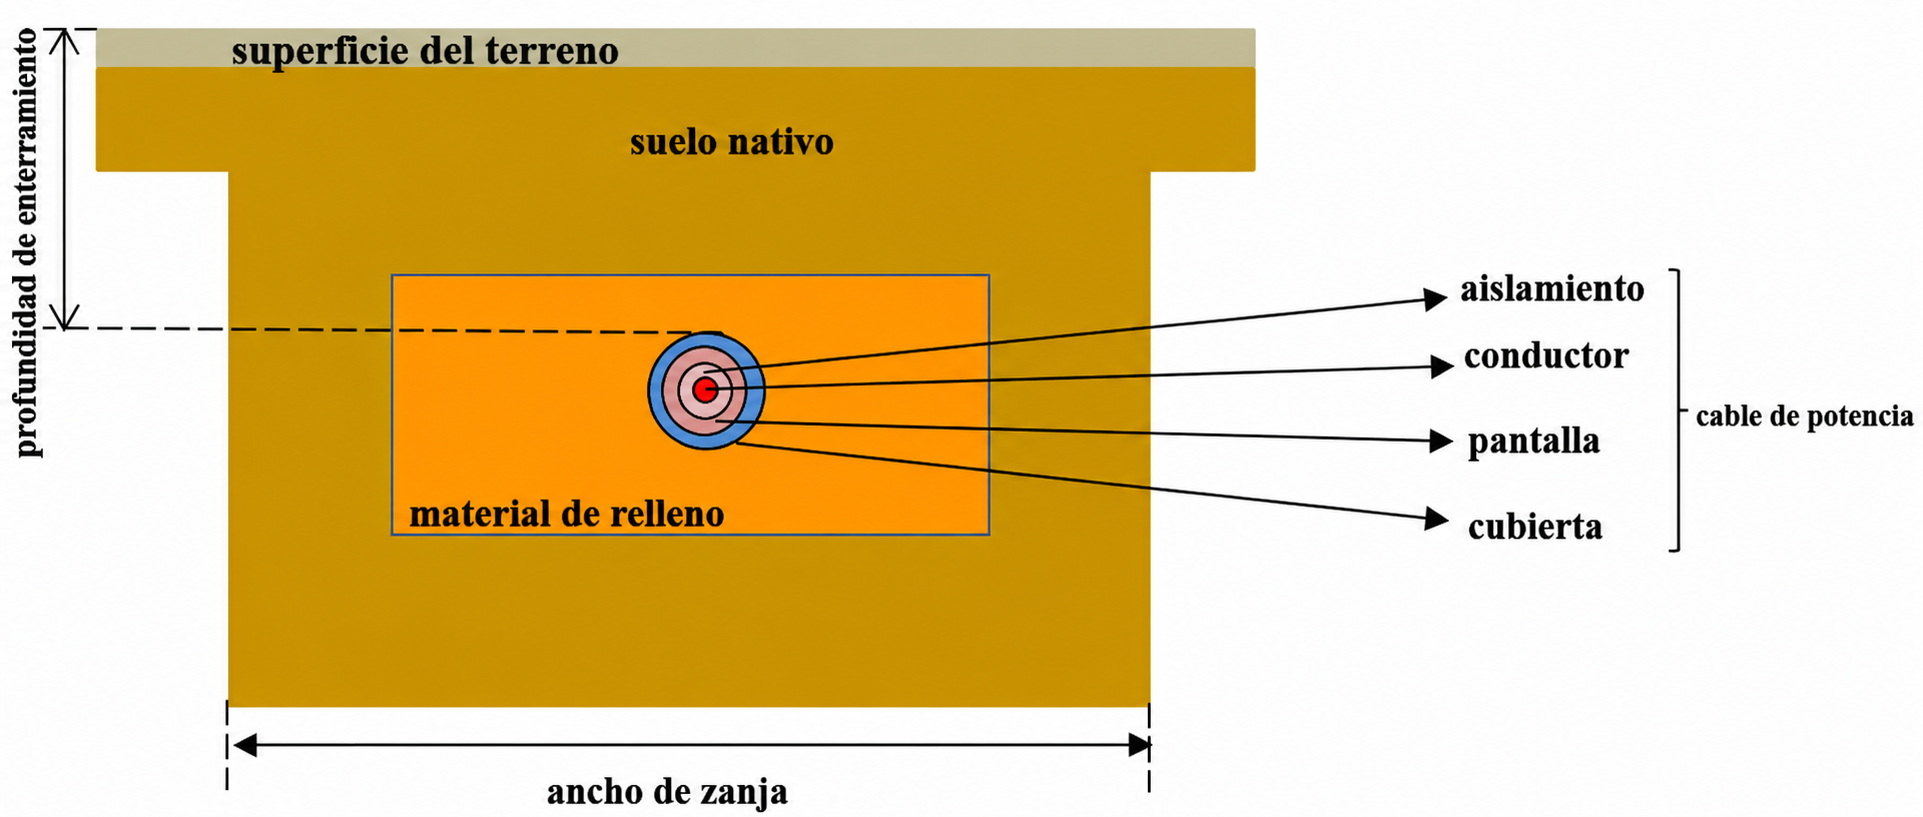
\includegraphics[width=0.96\textwidth,height=6.8cm,keepaspectratio]{enescu_trench_xsection_es.png}
\caption[Zanja y entorno térmico del cable enterrado]{Zanja y entorno térmico del cable enterrado. Fuente: Elaboración propia a partir de \textcite[fig.~1]{enescu2021}.}
\label{fig:zanja-cable}
\end{figure}

\subsection{ECUACIÓN DE CONDUCCIÓN Y CONDICIONES AUXILIARES}

La ecuación transitoria incorpora la capacidad térmica volumétrica y permite representar la evolución temporal. Para una sección 2D con propiedades espaciales, la ecuación puede escribirse como una adaptación de la ecuación clásica de calor \parencites{carslaw1959conduction,kakac2018heatConduction,hahn2012heatConduction}:

\begin{formula}[htbp]
\centering
\begin{equation}
\label{for:calor-transitorio}
\rho(x,y)c_p(x,y)\frac{\partial T(x,y,t)}{\partial t}
=\nabla\!\cdot\!\left(k(x,y)\nabla T(x,y,t)\right)+Q(x,y,t).
\end{equation}
\caption{Ecuación de conducción de calor 2D transitoria.}
\end{formula}

En la Fórmula~\ref{for:calor-transitorio}, $\rho c_p$ representa la capacidad térmica volumétrica, $k$ controla la conducción local y $Q$ agrupa las fuentes internas. El régimen transitorio queda fuera del alcance principal, pero la ecuación permite identificar la simplificación adoptada.

En régimen estacionario se anula la acumulación térmica. La formulación central del estudio se expresa en la Fórmula~\ref{for:calor-estacionario} \parencites{carslaw1959conduction,kakac2018heatConduction}[3]{xing2023}.

\begin{formula}[htbp]
\centering
\begin{equation}
\label{for:calor-estacionario}
\nabla\!\cdot\!\left(\kx\nabla T(x,y)\right)+Q(x,y)=0,
\qquad (x,y)\in\Omega.
\end{equation}
\caption{Ecuación de conducción de calor 2D estacionaria.}
\end{formula}

La Fórmula~\ref{for:calor-estacionario} conserva $\kx$ dentro del operador diferencial. Esta forma permite representar discontinuidades entre materiales sin sustituirlas por una propiedad global.

Las interfaces deben conservar temperatura y flujo normal, salvo que el caso declare una resistencia de contacto. La Fórmula~\ref{for:interfaces} formaliza ambas condiciones \parencites{carslaw1959conduction,kakac2018heatConduction}{patankar1980numerical}[3]{xing2023}.

\begin{formula}[htbp]
\centering
\begin{equation}
\label{for:interfaces}
T_1=T_2,
\qquad
\mathbf{n}\cdot k_1\nabla T_1=\mathbf{n}\cdot k_2\nabla T_2
\quad\text{en }\Gamma_{12}.
\end{equation}
\caption{Condiciones de continuidad térmica en una interfaz.}
\end{formula}

La Fórmula~\ref{for:interfaces} evita saltos no físicos entre materiales. El borde exterior puede usar temperatura prescrita, flujo o una condición convectiva equivalente, según la referencia elegida.

\subsection{CONDUCTIVIDAD, RESISTIVIDAD Y HETEROGENEIDAD}

La conductividad térmica $k$ expresa la facilidad para transferir calor. La resistividad $\rhoth$ expresa la oposición a esa transferencia. En un material homogéneo e isotrópico son magnitudes inversas, como muestra la Fórmula~\ref{for:k-rho}.

\begin{formula}[htbp]
\centering
\begin{equation}
\label{for:k-rho}
\rhoth=\frac{1}{k},\qquad k=\frac{1}{\rhoth}.
\end{equation}
\caption{Relación entre conductividad y resistividad térmica.}
\end{formula}

La Fórmula~\ref{for:k-rho} permite convertir los valores publicados antes de parametrizar el modelo. En suelos, estas propiedades dependen de composición, densidad y contenido de agua. Los valores empleados para diseño deben representar el estado de la instalación y seguir procedimientos normalizados cuando proceden de ensayos \parencites{farouki1981thermal,devries1966thermal}[secciones~4--6]{ieee442}.

La heterogeneidad se caracteriza mediante el contraste de conductividad, el patrón espacial, la extensión de la región y su proximidad al conductor. Estas dimensiones describen la física de los casos y deben variar de forma controlada durante las comparaciones pareadas.

\subsection{TEMPERATURA MÁXIMA Y AMPACIDAD}

La ampacidad no es una propiedad fija del cable aislado. Cambia con la temperatura ambiente, la profundidad, la separación, la configuración, las pérdidas y el estado térmico del terreno \parencites[3--6]{enescu2021}[1,6--9]{khumalo2025}. La condición operacional usada en el estudio se expresa en la Fórmula~\ref{for:ampacidad}.

\begin{formula}[htbp]
\centering
\begin{equation}
\label{for:ampacidad}
\Imax=\max\left\{I:\max_{(x,y)\in\Omega_c}T(x,y;I)\leq T_{\mathrm{lim}}\right\}.
\end{equation}
\caption{Condición operacional para calcular la ampacidad.}
\end{formula}

La Fórmula~\ref{for:ampacidad} define $\Imax$ como la mayor corriente que mantiene la temperatura máxima del conductor por debajo del límite adoptado. Por tanto, la calidad del cálculo de ampacidad depende de la calidad del campo $T(x,y;I)$ y de la representación de las pérdidas.

\subsection{MÉTODOS DE CÁLCULO TÉRMICO}

Los circuitos térmicos son rápidos e interpretables, pero requieren equivalencias geométricas. FEM, FDM y FVM resuelven la ecuación sobre una discretización y pueden representar materiales y contornos con mayor detalle. Su credibilidad depende de las propiedades, la discretización, la convergencia y la verificación \parencites{patankar1980numerical}[3--4,93--99]{cigre2025}.

Las PINN aproximan la solución con una red neuronal y diferenciación automática. No eliminan la necesidad de especificar la física; trasladan parte de la dificultad al muestreo, la ponderación de pérdidas y la optimización \parencites[686--690]{raissi2019}[1--2,14--17]{lawal2022}. La Tabla~\ref{tab:metodos-termicos} resume el papel previsto de cada enfoque.

\begin{table}[htbp]
\centering
\caption{Papel de los métodos térmicos dentro de la investigación. Fuente: Elaboración propia.}
\label{tab:metodos-termicos}
\begin{tabularx}{\textwidth}{L{2.5cm}Y Y}
\toprule
\textbf{Método} & \textbf{Fortaleza y límite relevante} & \textbf{Uso en la investigación} \\
\midrule
IEC/circuital & Cálculo interpretable con resistencias equivalentes; representación espacial limitada. & Línea base normativa cuando el caso sea comparable. \\
Analítico o manufacturado & Respuesta conocida y trazable; geometría normalmente simple. & Verificación elemental de formulación y código. \\
FEM & Geometría y materiales explícitos; requiere malla y estudio de convergencia. & Referencia numérica independiente del campo térmico. \\
PINN & Aproximación continua y física incorporada; entrenamiento sensible a muestreo y pérdidas. & Artefacto principal investigado. \\
\bottomrule
\end{tabularx}
\end{table}

Los métodos se consideran complementarios. Una discrepancia no implica por sí sola que IEC sea insuficiente o que la PINN sea superior. Primero deben compararse los supuestos, el dominio y la calidad de la evidencia.

\subsection{RED NEURONAL INFORMADA POR FÍSICA}

Una PINN representa la temperatura mediante una red $T_\theta(x,y)$. La diferenciación automática permite evaluar derivadas espaciales y construir residuos de la PDE, los contornos y las interfaces \parencite[686--690]{raissi2019}. La función de pérdida lógica se muestra en la Fórmula~\ref{for:perdida-pinn}.

\begin{formula}[htbp]
\centering
\begin{equation}
\label{for:perdida-pinn}
\mathcal{L}(\theta)=
w_f\mathcal{L}_{\mathrm{PDE}}+
w_b\mathcal{L}_{\mathrm{cont}}+
w_i\mathcal{L}_{\mathrm{int}}+
w_d\mathcal{L}_{\mathrm{datos}}+
w_e\mathcal{L}_{\mathrm{energía}}.
\end{equation}
\caption{Función de pérdida lógica del artefacto PINN.}
\end{formula}

La Fórmula~\ref{for:perdida-pinn} reúne restricciones físicas y datos de referencia cuando existen. Los pesos no se consideran universales, porque un balance inadecuado de gradientes puede sesgar el entrenamiento \parencites[16]{pan2025}[1--2,17]{lawal2022}.

La Figura~\ref{fig:flujo-pinn} organiza el flujo lógico. Las entradas físicas alimentan la red; la diferenciación automática genera residuos; y el optimizador actualiza los parámetros hasta cumplir los criterios definidos.

\begin{figure}[htbp]
\centering
\resizebox{0.96\textwidth}{!}{%
\begin{tikzpicture}[
  bloque/.style={draw,rounded corners=3pt,align=center,text width=3.0cm,minimum height=1.15cm,font=\small},
  arr/.style={-{Stealth[length=2.7mm]},thick}]
\node[bloque,fill=lightblue] (in) {Entradas\\$(x,y)$, $k$, $Q$\\contornos e interfaces};
\node[bloque,fill=lightgray,right=0.7cm of in] (nn) {Red PINN\\$T_\theta(x,y)$};
\node[bloque,fill=green!12,right=0.7cm of nn] (ad) {Diferenciación\\automática};
\node[bloque,fill=orange!14,right=0.7cm of ad] (loss) {Residuos y\\pérdida total};
\node[bloque,fill=red!8,below=0.8cm of ad] (out) {Campo térmico\\$T(x,y)$, $\Tmax$, $\Imax$};
\node[bloque,fill=yellow!15,below=0.8cm of loss] (opt) {Optimizador\\actualiza $\theta$};
\draw[arr] (in)--(nn);
\draw[arr] (nn)--(ad);
\draw[arr] (ad)--(loss);
\draw[arr] (loss)--(opt);
\draw[arr] (opt.west)-| (nn.south);
\draw[arr] (ad)--(out);
\end{tikzpicture}}
\caption{Flujo lógico de una PINN aplicada a conducción de calor. Fuente: Elaboración propia a partir de \textcite{raissi2019}, \textcite{lawal2022} y \textcite{pan2025}.}
\label{fig:flujo-pinn}
\end{figure}

\subsection{CIENCIA DEL DISEÑO Y NATURALEZA DE LA CONTRIBUCIÓN}

DSR produce conocimiento prescriptivo mediante artefactos útiles y evaluados. El artefacto situado es el prototipo PINN aplicado al arreglo de cables--entorno térmico. La contribución abstracta prevista comprende requisitos, arquitectura, protocolo de evaluación, límites y principios de diseño \parencite[343--349]{gregor2013}.

Los principios iniciales consisten en conservar la física, representar interfaces sin promedios inadvertidos, separar verificación de validación, mantener la incertidumbre numérica por debajo del efecto analizado y preservar la trazabilidad. Son proposiciones sujetas a evaluación, no conclusiones anticipadas.

\section{DEFINICIÓN DE TÉRMINOS}
\label{sec:definicion-terminos}

\begin{description}[style=nextline,itemsep=0.5\baselineskip]
  \item[Ampacidad.] Corriente máxima que puede transportar un cable sin superar el límite térmico adoptado para sus materiales y condiciones de instalación. Se denota $\Imax$ \parencites{iec60287}[3--6]{enescu2021}.

  \item[Arreglo de cables--entorno térmico.] Objeto físico formado por los cables, su disposición, el lecho de asiento, el relleno, el suelo nativo, las fuentes y los contornos.

  \item[Artefacto.] Producto diseñado para resolver un problema relevante y generar conocimiento evaluable. En esta investigación comprende especificación, prototipo, escenarios, métricas y principios derivados \parencites{peffers2007}{gregor2013}.

  \item[Campo de temperatura.] Distribución espacial $T(x,y)$ en la sección 2D. Permite derivar $\Tmax$, la ubicación del punto caliente y $\Imax$.

  \item[Ciencia del diseño (DSR).] Paradigma que organiza el diseño, demostración y evaluación de artefactos orientados a problemas prácticos \parencites{peffers2007}{gregor2013}.

  \item[Condición de contorno.] Restricción aplicada en el borde del dominio, como temperatura, flujo o intercambio convectivo equivalente.

  \item[Conductividad térmica.] Propiedad $k$, expresada en \si{\watt\per\metre\per\kelvin}, que mide la facilidad de un material para conducir calor.

  \item[Contraste de conductividad.] Relación entre la conductividad de una región heterogénea y la del material base.

  \item[FEM.] Método de elementos finitos usado como referencia numérica convergente del campo, no como artefacto principal.

  \item[Heterogeneidad térmica.] Variación espacial de propiedades térmicas. El estudio se centra en $\kx$ y en su contraste, patrón, extensión y proximidad.

  \item[Interfaz térmica.] Frontera interna entre materiales. El modelo exige continuidad de temperatura y de flujo normal, salvo que se declare resistencia de contacto.

  \item[PINN.] Red neuronal informada por física que aproxima una variable física y penaliza el incumplimiento de la PDE y de condiciones auxiliares \parencite{raissi2019}.

  \item[Punto caliente.] Ubicación donde el campo alcanza la máxima temperatura relevante para el conductor o la operación.

  \item[Representación homogénea equivalente.] Sustitución de un entorno heterogéneo por una propiedad térmica única usada como referencia de comparación.

  \item[Residuo físico.] Incumplimiento local de la ecuación gobernante o de una condición auxiliar al evaluar $T_\theta(x,y)$.

  \item[Resistividad térmica.] Propiedad $\rhoth$, expresada en \si{\kelvin\metre\per\watt}, que mide la oposición a la conducción y es la inversa de $k$.

  \item[Solución manufacturada.] Solución definida de antemano para construir fuentes y contornos compatibles y verificar el error del código.

  \item[Temperatura máxima del conductor.] Máximo de $T(x,y)$ en la región del conductor, denotado $\Tmax$.

  \item[Validación.] Evaluación de si el modelo representa una instalación real mediante evidencia empírica independiente. La validación experimental queda fuera del alcance.

  \item[Verificación.] Evaluación de si la formulación y el código resuelven correctamente el problema especificado mediante referencias y balances.

  \item[XLPE.] Polietileno reticulado usado como aislamiento en cables de potencia. Su límite térmico condiciona la corriente admisible \parencite{iec60502_2_2014}.
\end{description}

En síntesis, la cadena física parte de $\kx$, continúa con el flujo y el campo térmico, y termina en $\Tmax$ e $\Imax$. El Capítulo~\ref{ch:propuesta-desarrollo} transforma esta cadena en la arquitectura del artefacto, su desarrollo y la evidencia que todavía debe producirse.


\chapter{PROPUESTA Y DESARROLLO DE LA SOLUCIÓN}
\label{ch:propuesta-desarrollo}

Este capítulo presenta la formulación explícita, el diseño experimental registrado antes de la búsqueda, sus resultados y el dominio de aceptación. Las campañas anteriores de suelo perforado y reconstrucción radial se conservan en el expediente histórico, pero no se suman a los resultados de esta formulación. Cambiar la física obliga a producir nuevas referencias FEM y a recalificar las redes.

\section{PRESENTACIÓN DE LA PROPUESTA DE SOLUCIÓN}
\label{sec:presentacion-propuesta}

El artefacto comprende un contrato físico común, un solucionador PINN, una referencia independiente FEniCSx y un expediente por ejecución. La temperatura se calcula dentro del conductor, aislamiento, pantalla, cubierta y suelo. Cada región tiene su ecuación diferencial y las interfaces transmiten temperatura y flujo. No se prescribe una potencia uniforme en la superficie exterior del cable ni se añade una caída térmica resistiva para obtener la temperatura central.

La contribución de ciencia del diseño reside en el procedimiento de especificación, elección, verificación y delimitación del artefacto. La aprobación del protocolo autoriza la experimentación, pero no acredita automáticamente todas las redes o casos. Una red se entrena para cada problema; no se ha demostrado un operador que generalice sin reentrenamiento a geometrías y parámetros nuevos \parencites{peffers2007}{gregor2013}.

\section{DESARROLLO DE LA PROPUESTA DE SOLUCIÓN}
\label{sec:desarrollo-solucion}

\subsection{CONTRATO FÍSICO Y FUENTES DE DATOS}

Los archivos JSON UTF-8 definen el caso físico: dominio, centros, radios y espesores, conductividad de cada material, ley espacial del suelo, corriente, resistencia, coeficiente térmico, contornos y procedencia. Las longitudes se expresan en metros; $k$ en \si{\watt\per\metre\per\kelvin}; $Q$ en \si{\watt\per\metre\cubed}; la potencia lineal en \si{\watt\per\metre}; las diferencias de temperatura en kelvin. Los hiperparámetros y las semillas pertenecen a otro archivo y no alteran la identidad física del problema.

Los cables del catálogo emplean el rectángulo $[-4,4]\times[-4,0]$ m y temperatura exterior prescrita de 20 °C. Este contorno finito forma parte del caso; la convergencia de malla no demuestra independencia respecto a la extensión del terreno. El control coaxial utiliza un círculo de radio 0,15 m. Su versión angular prescribe $T=20+10x$ en el contorno, con $x$ en metros. Este último problema evita elegir una representación únicamente por su desempeño en simetría radial.

La familia XLPE tiene radio de conductor de 5,5 mm y radio exterior de 15 mm. Incluye suelo homogéneo, estratos con salto exacto, relleno mejorado y zonas de baja conductividad cercana y lejana. Aras incorpora un arreglo plano de tres cables; Kim incorpora seis cables en arena. Las geometrías se apoyan en \textcite{aras2005} y \textcite{kim2025}, pero el dominio, las fuentes y los contornos controlados no reproducen íntegramente sus instalaciones. El año 2024 en carpetas Kim identifica una convención histórica; la referencia bibliográfica es de 2025. El coeficiente DC adoptado es $0,00393\ \mathrm{K}^{-1}$, documentando la discrepancia con el valor $0,0393$ impreso en la fuente utilizada anteriormente.

Una transición de suelo suavizada y una interfaz con salto exacto son problemas distintos. Su ancho se registra como propiedad del caso, sin ajustarlo para facilitar el entrenamiento. Se rechazan geometrías superpuestas, capas discontinuas en radio, propiedades no positivas y estratos que atraviesen un cable cuando el generador geométrico no admite esa intersección.

La resistencia eléctrica debe identificar base DC o AC, frecuencia, temperatura y fuente primaria. Los datos históricos denominados R20 se tratan como DC para los controles declarados; el nombre no certifica por sí solo la naturaleza del dato original. La campaña principal compara fuentes prescritas. La ley DC local y el cálculo de corriente límite se evalúan por separado. No se transfieren cifras históricas de ampacidad reducida al modelo explícito.

\begingroup\footnotesize\setlength{\tabcolsep}{3pt}
\begin{longtable}{L{4.2cm}rrrrr}
\caption{Entradas eléctricas y del suelo base de la campaña a fuente prescrita. Fuente: contratos de caso documentados.}\label{tab:explicit-case-inputs}\\
\toprule
Caso & Cables & I, A & $R_{20}$, $\Omega$/km & P por cable, W/m & k base, W/(m K)\\
\midrule\endfirsthead
\toprule
Caso & Cables & I, A & $R_{20}$, $\Omega$/km & P por cable, W/m & k base, W/(m K)\\
\midrule\endhead
coaxial\_angular & 1 & 270 & 0.19300 & 14.06970 & 1.000\\
xlpe\_single & 1 & 270 & 0.19300 & 14.06970 & 1.000\\
xlpe\_discrete\_layers & 1 & 270 & 0.19300 & 14.06970 & 1.000\\
xlpe\_backfill & 1 & 270 & 0.19300 & 14.06970 & 1.000\\
xlpe\_dry\_near & 1 & 270 & 0.19300 & 14.06970 & 1.000\\
xlpe\_dry\_far & 1 & 270 & 0.19300 & 14.06970 & 1.000\\
aras\_flat & 3 & 1110 & 0.01510 & 18.60471 & 1.000\\
kim\_sand & 6 & 1026 & 0.01510 & 15.89541 & 1.365\\
\bottomrule\end{longtable}\endgroup

\begingroup\footnotesize\setlength{\tabcolsep}{3pt}
\begin{longtable}{L{4.2cm}rrrrr}
\caption{Capas explícitas: índice cero conductor, los restantes materiales pasivos. Fuente: fichas de entrada auditadas.}\label{tab:explicit-layers}\\
\toprule
Familia & Capa & $r_i$, mm & $r_o$, mm & Espesor, mm & k, W/(m K)\\
\midrule\endfirsthead
\toprule
Familia & Capa & $r_i$, mm & $r_o$, mm & Espesor, mm & k, W/(m K)\\
\midrule\endhead
xlpe\_single & 0 & 0.00 & 5.50 & 5.50 & 400\\
xlpe\_single & 1 & 5.50 & 12.00 & 6.50 & 0.286\\
xlpe\_single & 2 & 12.00 & 13.00 & 1.00 & 380\\
xlpe\_single & 3 & 13.00 & 15.00 & 2.00 & 0.45\\
aras\_flat & 0 & 0.00 & 18.85 & 18.85 & 400\\
aras\_flat & 1 & 18.85 & 40.85 & 22.00 & 0.2857\\
aras\_flat & 2 & 40.85 & 49.35 & 8.50 & 384.6\\
aras\_flat & 3 & 49.35 & 53.35 & 4.00 & 0.45\\
kim\_sand & 0 & 0.00 & 21.20 & 21.20 & 400\\
kim\_sand & 1 & 21.20 & 23.20 & 2.00 & 0.2857\\
kim\_sand & 2 & 23.20 & 40.20 & 17.00 & 0.2857\\
kim\_sand & 3 & 40.20 & 41.50 & 1.30 & 0.2857\\
kim\_sand & 4 & 41.50 & 42.50 & 1.00 & 0.167\\
kim\_sand & 5 & 42.50 & 45.00 & 2.50 & 237\\
kim\_sand & 6 & 45.00 & 50.00 & 5.00 & 0.2857\\
kim\_sand & 7 & 50.00 & 100.00 & 50.00 & 2.15\\
kim\_sand & 8 & 100.00 & 110.00 & 10.00 & 0.2857\\
\bottomrule\end{longtable}\endgroup

Los casos coaxial y XLPE comparten la secuencia radial de XLPE. El centro coaxial es (0,0); XLPE está en (0,−0,7) m. Aras utiliza centros (−0,33;−1,2), (0;−1,2) y (0,33;−1,2) m. Kim utiliza x=−0,4, 0 y 0,4 m en dos filas y=−1,6 y −1,2 m. Las capas de Kim se conservan individualmente aunque algunas tengan igual conductividad. No se homogeneiza su difusión térmica.

Las zonas suaves emplean $k(x,y)=k_0+(k_p-k_0)S_\varepsilon(x;c_x,w)S_\varepsilon(y;c_y,h)$, donde $S_\varepsilon(s;c,w)=\tfrac12[\tanh((s-c+w/2)/\varepsilon)-\tanh((s-c-w/2)/\varepsilon)]$. El mapa se evalúa únicamente en suelo; las capas conservan su k.

\begingroup\footnotesize\setlength{\tabcolsep}{3pt}
\begin{longtable}{L{4.2cm}rrrrrr}
\caption{Definición de heterogeneidades suaves del suelo. Fuente: casos registrados.}\label{tab:explicit-patches}\\
\toprule
Caso & $c_x$, m & $c_y$, m & w, m & h, m & $k_p$ & $\varepsilon$, m\\
\midrule\endfirsthead
\toprule
Caso & $c_x$, m & $c_y$, m & w, m & h, m & $k_p$ & $\varepsilon$, m\\
\midrule\endhead
xlpe\_backfill & 0 & -0.7 & 0.5 & 0.5 & 2 & 0.08\\
xlpe\_dry\_near & 0 & -0.7 & 0.5 & 0.5 & 0.5 & 0.08\\
xlpe\_dry\_far & 1 & -0.7 & 0.5 & 0.5 & 0.5 & 0.08\\
\bottomrule\end{longtable}\endgroup

Los estratos emplean k=0,5 W/(m K) bajo y=−1 m y k=1 W/(m K) sobre esa interfaz, con salto exacto. Los demás casos de esta tabla no tienen bandas adicionales. Las resistencias de los controles se interpretan como DC a 20 °C; el coeficiente térmico es 0,00393 $\mathrm{K}^{-1}$. La frase histórica «flujo circular uniforme» que subsiste en la procedencia del catálogo describe su uso anterior; el contrato explícito y la pérdida activa utilizan generación volumétrica y transmisión entre materiales.


\subsection{ECUACIONES Y REPRESENTACIÓN MULTIESCALA}

La PDE estacionaria por material es $-\nabla\cdot(k_i\nabla T_i)=Q_i$. En el conductor $Q_i$ es volumétrica; en capas pasivas y suelo es cero. Se conservan las derivadas de $k(x,y)$ dentro de regiones continuas. Una misma normal define continuidad de $T$ y de $\mathbf q\cdot\mathbf n$ en cada interfaz. El borde exterior Dirichlet se impone mediante la función de aproximación.

Los anillos usan la coordenada logradial y las entradas periódicas descritas en el Capítulo II. La red del conductor usa cartesianas normalizadas por su radio. El suelo conserva coordenadas globales normalizadas y distancias locales a cables. Las derivadas se calculan respecto a las coordenadas físicas, por lo que no se pierden los factores de escala. La transformación de entradas no convierte el problema general en una ecuación radial de una sola variable.

Cada subred de temperatura produce una corrección con escala térmica local y un desplazamiento entrenable. Para una red de temperatura y flujo se calculan ambas variables. El flujo aprendido satisface la ley de Fourier tanto en el interior como en las trazas de interfaz y contorno. La aceptación comprueba, además, el flujo calculado directamente de $-k\nabla T$; aceptar solo un flujo auxiliar podría ocultar un campo térmico inconsistente.

\begin{formula}[htbp]
\begin{equation}
\mathcal L=\mathcal L_{\mathrm{PDE}}+\mathcal L_{\mathrm{constitutiva}}
+w_T\mathcal L_{[T]}+10\mathcal L_{[q_n]}+10\mathcal L_{\mathrm{energía}}.
\label{for:perdida-explicita}
\end{equation}
\caption{Pérdida adimensional común de la campaña explícita.}
\end{formula}

El término constitutivo solo aparece cuando el flujo es una salida independiente. La energía se integra por región, con fuentes y flujos calculados; no se reemplaza el flujo obtenido por la potencia prescrita para imponer artificialmente un balance nulo. Las medias de los residuos se calculan por material, de modo que un aislamiento pequeño no desaparezca por ponderación de área. A--C mantienen $w_T=100$ y los demás pesos fijos. La calibración C2 varía únicamente $w_T$ antes de la confirmación; así la comparación de arquitectura no se confunde con cambiar simultáneamente la función objetivo. Las temperaturas FEM no intervienen en la pérdida.

\subsection{REFERENCIA FEM Y PUERTA DE DISCRETIZACIÓN}

FEniCSx 0.10.0 y Gmsh 4.15.2 resuelven una partición geométrica conforme con elementos triangulares P2 y geometría curva. Cada capa tiene una etiqueta de integración y su propia conductividad. La fuente se integra en el conductor; las interfaces son internas a la malla. PETSc/MUMPS resuelve el sistema y la falta de convergencia interrumpe la referencia \parencite{baratta2023dolfinx}.

Se ejecutan al menos tres mallas y hasta cinco si es necesario. El refinamiento reduce el tamaño local según el espesor de cada capa y mantiene resolución del suelo. La puerta exige, entre las dos últimas mallas, cambio de Tmax menor a 0,1 K y a 0,5\,\pct{} de la elevación térmica, RMSE de cambio por región menor a 0,5\,\pct{} de esa elevación y balance exterior menor a 0,2\,\pct{}. Son umbrales de discretización más estrictos que la aceptación PINN. El cambio entre mallas es evidencia de convergencia observada y no una cota rigurosa del error desconocido.

La evaluación independiente contiene 512 puntos por región, incluido el centro del conductor. Se informan errores por material y un RMSE ponderado por área. La localización FEM selecciona primero el material y después la celda mediante coordenadas isoparamétricas. Una primera celda candidata incorrecta en una interfaz curva produjo errores espurios durante el piloto; ese defecto se corrigió antes de generar las referencias de esta campaña. Los campos se comparan en puntos idénticos y con identidad física SHA-256 coincidente.

En el control coaxial simétrico se dispone también de una solución analítica de Poisson/Laplace. Se usa exclusivamente para verificación externa. La referencia P2 fina obtuvo un error de Tmax de aproximadamente $3,68\times10^{-6}$ K. Una identidad analítica en ese caso no sustituye la comprobación FEM de los casos angulares y heterogéneos.

\subsection{SELECCIÓN DE ARQUITECTURA Y TAMAÑO}
\label{sec:seleccion-pinn}

La búsqueda distingue formulación, representación y tamaño. Se comparan redes de temperatura por material, redes mixtas de temperatura y flujo, entradas cartesianas locales, entradas Fourier y enriquecimiento multipolar. Los alias \texttt{enriched}, \texttt{conservative} y \texttt{subdomain} de la implementación explícita no constituyen tres métodos diferentes. La red global suave se considera un control negativo por la incompatibilidad de sus derivadas normales en una interfaz con salto de k y flujo no nulo.

La formulación mixta es equivalente a la ecuación de calor y se relaciona con la motivación de FO-PINNs \parencite{gladstone2022fopinn}; no se presenta como reproducción exacta del artículo. Los armónicos multipolares son funciones de enriquecimiento entrenables, regulares dentro del conductor. La variante implementada usa enriquecimiento exterior respecto al primer cable, lo que limita su simetría en arreglos múltiples y debe tenerse en cuenta al interpretar sus resultados. VPINN, descomposición con ventanas solapadas y ponderación adaptativa de gradientes son alternativas bibliográficas, no resultados adicionales de esta campaña \parencites{kharazmi2020hpvpinn}{moseley2021fbpinn}{wang2020gradients}.

La etapa A compara nueve configuraciones: temperatura por subdominios de 8×2, 16×2, 16×3 y 32×3; mixta de 16×2 y 32×3; y local, Fourier y multipolar de 16×2. La notación indica anchura y número de capas ocultas por material. Se utiliza tangente hiperbólica, inicialización reproducible y precisión doble. Todos los candidatos reciben Adam con 1200 pasos, tasa $10^{-3}$ y hasta 2000 iteraciones L-BFGS con búsqueda lineal. Se registran sus evaluaciones reales, que no necesariamente coinciden con el límite de iteraciones.

Los problemas de desarrollo de A son el coaxial angular y el XLPE homogéneo. Las semillas de inicialización 11 y 23 se combinan con semillas de muestreo 101 y 103, respectivamente; se conserva la pareja en cada alternativa. Esto permite comparaciones pareadas, pero no separa estadísticamente ambos componentes de variación. El presupuesto inicial es de 256 puntos por región de suelo, 128 por capa del cable y 96 por interfaz.

La regla prioriza candidatos aceptados en los dos problemas y las dos semillas. Entre ellos se elige el menor número de parámetros entrenables; a igual tamaño se prefiere menor peor error normalizado. Si ninguno cumple, se registra una selección provisional por cantidad de aceptaciones y menor máxima violación de las tolerancias. Tal selección no demuestra una red mínima admisible. Un rechazo con entrenamiento finito tampoco prueba insuficiencia matemática de una arquitectura por material.

La búsqueda es preliminar y discreta. No cubre todas las anchuras, profundidades, activaciones y combinaciones de entrenamiento. La literatura sobre optimización de hiperparámetros advierte que el resultado depende del espacio explorado y del presupuesto \parencite{bergstra2012random}. Por ello se utiliza la expresión ``menor red admisible entre las ensayadas'', y únicamente cuando la evidencia permita sostenerla.

\subsection{CONVERGENCIA Y DISTRIBUCIÓN DE COLOCACIONES}
\label{sec:analisis-numerico-pinn}
\label{sec:muestreo-adaptativo}

La etapa B conserva la arquitectura seleccionada y compara el XLPE homogéneo con el XLPE de dos estratos discontinuos. El segundo añade una interfaz plana de suelo y permite evaluar si la regla obtenida en una geometría más simple se transfiere. Se mantienen las dos parejas de semillas de desarrollo.

La mezcla geométrica combina una mitad de muestras de cobertura global con una mitad próxima a los cables. Se ejecutan presupuestos 1×, 2× y 4×, escalando los puntos por región e interfaz. En el presupuesto 2× se comparan además distribución uniforme, bandas de interfaz y adaptación por residuo. Por tanto, el análisis separa aumentar el número de puntos de cambiar su ubicación manteniendo el número. Se informan las cantidades efectivas: el parámetro de suelo no es el total del problema.

Las bandas de interfaz conservan una mitad uniforme y concentran la otra cerca de las caras de las capas, la superficie del conductor y los saltos del suelo. La política adaptativa genera cuatro veces el número de candidatos por región y usa el residuo adimensional de la PDE. En la red mixta agrega el defecto constitutivo. Al alcanzar la mitad de Adam selecciona sin reemplazo una mitad del presupuesto según probabilidades proporcionales al indicador, con un término positivo que evita excluir completamente candidatos de residuo pequeño. La otra mitad mantiene cobertura uniforme. L-BFGS utiliza después una nube fija.

Esta adaptación se fundamenta en las estrategias de \textcite{wu2022sampling}, pero no se declara una reproducción exacta de RAD. El muestreo sesgado modifica la medida efectiva de la pérdida porque no se aplica corrección por importancia. Las fronteras e interfaces mantienen cuadraturas uniformes para calcular balances; concentrar puntos de control no autoriza a interpretar una media no ponderada como integral uniforme. La referencia FEM y la evaluación final permanecen independientes de la selección de colocaciones.

\begin{formula}[htbp]
\begin{equation}
D_{N,2N}=100\frac{\sqrt{\sum_j w_j(T_N-T_{2N})^2/\sum_j w_j}}
{|T^F_{\max}-T_0|},\qquad
H_{N,2N}=100\frac{|T_{\max,N}-T_{\max,2N}|}{|T^F_{\max}-T_0|}.
\label{for:insensibilidad-explicita}
\end{equation}
\caption{Indicadores de insensibilidad observada al aumentar colocaciones.}
\end{formula}

Se examinan diferencias de campo, Tmax y errores por material frente a FEM. Valores inferiores a 0,5\,\pct{} en $D$ y $H$, junto con aceptación de ambas soluciones, apoyan insensibilidad en el intervalo ensayado. Si no se cumple, se informa dependencia de la resolución aunque una corrida aislada alcance el umbral de 5\,\pct{}. Dos soluciones igualmente sesgadas pueden parecer estables; por eso se conserva la comparación externa.

La pendiente empírica de error frente a N es descriptiva. No constituye un orden teórico de convergencia PINN ni justifica extrapolación de Richardson sobre neuronas o colocaciones. Los errores de aproximación, cuadratura/generalización del residuo y optimización tienen contribuciones distintas \parencites{deryck2024analysis}{mishra2020error}. Las nubes no se presentan como mallas anidadas deterministas. La comparación entre semillas permite observar variación, sin convertir dos repeticiones en una garantía estadística.

La política de menor presupuesto aceptado se selecciona con los casos de B. La comparación 1×--2×--4× determina si además puede calificarse como insensible dentro del rango probado. El hecho de que un presupuesto sea admisible no permite llamarlo automáticamente convergente. No se ensaya 10× por regla general: se requiere una razón física o numérica para ese coste adicional.

\subsection{AJUSTE DEL ENTRENAMIENTO Y CONFIRMACIÓN}

La etapa C conserva arquitectura y colocaciones y compara tasas Adam $5\times10^{-4}$, $10^{-3}$ y $2\times10^{-3}$, con 1500 pasos y hasta 3000 iteraciones L-BFGS. Se usan los dos problemas y parejas de semillas de B. La selección prioriza aceptación completa y menor peor violación de los criterios. Cambiar simultáneamente el presupuesto entre A y C se interpreta como una etapa de ajuste posterior, no como un efecto aislado de tasa de aprendizaje; dentro de C el presupuesto sí es común.

Durante B se registró una ampliación C2, antes de ejecutar C o D, motivada por saltos térmicos excesivos que persistían al aumentar puntos. La iteración formativa conserva la receta seleccionada en C y compara $w_T=100$, 1000 y 10000, sin cambiar PDE, normalizaciones ni tolerancias. El valor 100 reutiliza cuatro corridas de C; los otros dos añaden ocho entrenamientos con los mismos casos y semillas de desarrollo. Entre configuraciones completamente aceptadas se prefiere el menor peso; si ninguna cumple, se conservan la regla provisional de aceptación y máxima violación. El procedimiento se apoya en la necesidad de controlar el equilibrio de gradientes \parencite{wang2020gradients}, sin afirmar que implementa ponderación adaptativa.

La enmienda se declara como respuesta a evidencia de desarrollo, no como decisión original de A ni ajuste basado en confirmación. El total único es 101 entrenamientos A--D, incluidos los ocho de C2; se agregan nueve de corriente límite. El peso elegido en C2 forma parte de la receta congelada para D y para la extensión DC, que conserva el doble de presupuesto registrado.

Antes de la etapa D se congela la configuración y su huella. D utiliza semillas nuevas 71, 83 y 97, asociadas con muestreos 1001, 1003 y 1007. Se comparan XLPE homogéneo, estratos, relleno, zona seca cercana, zona seca lejana, Aras plano y Kim arena. Los dos primeros casos comprueban estabilidad con inicializaciones nuevas; los restantes evalúan transferencia de la receta a escenarios no usados para ajustarla. Se reentrena por caso, por lo que esa transferencia no equivale a generalización de pesos.

La etiqueta ``producción'' identifica el protocolo congelado, no una certificación operativa. Un resultado rechazado de D no se reemplaza por su mejor semilla ni se incorpora silenciosamente al ajuste. Una mejora posterior necesitaría otra ronda de desarrollo y nueva confirmación. Se publican mediana, rango y cantidad aceptada de todas las semillas, sin descartar resultados desfavorables.

\subsection{MÉTRICAS Y TRAZABILIDAD}

El denominador térmico es la elevación respecto al ambiente, no la temperatura Celsius absoluta. El RMSE global pondera el área representada por cada punto; cada material tiene además su RMSE propio. La puerta PINN exige NRMSE y error de elevación máxima no mayores a 5\,\pct{}, RMSE por material no mayor a 5\,\pct{} de la elevación de referencia, balances globales y por región no mayores a 2\,\pct{}, salto máximo de T no mayor a 0,1 K y salto RMS de flujo no mayor a 1\,\pct{} de la escala declarada. En la formulación mixta deben pasar tanto el flujo predicho como el derivado de T.

Para evitar ambigüedad, el balance global divide el defecto exterior entre la potencia total calculada de todos los conductores. El defecto de cada región se divide entre la potencia nominal por cable $P_0=I_0^2R_{20}$, también en capas pasivas donde la fuente local es cero. En ampacidad, $I_0$ es la corriente de referencia de la parametrización y esa escala se conserva aunque la corriente aprendida cambie. Por tanto, el porcentaje regional no usa como denominador la nueva pérdida eléctrica. El salto de flujo se divide entre la mayor escala de flujo de los dos materiales vecinos; el salto térmico se expresa directamente en kelvin.

Los umbrales se fijan antes de la confirmación y no se modifican para aceptar corridas. El balance usa flujos calculados. Se conservan puntos, regiones, pesos, fuentes, configuración, parámetros, estados de optimización, versiones y tiempos. Los JSON contienen la huella de física y de las fuentes del código. Las figuras y tablas se generan desde esos registros, evitando transcribir manualmente cifras entre resumen, resultados y conclusiones.

El equipo dispone de CPU Intel Core Ultra 7 165U y un acelerador Intel accesible mediante XPU, sin CUDA disponible. La campaña utiliza float64 y hasta tres procesos independientes con un hilo por entrenamiento. Se registran los recursos, pero los tiempos concurrentes no demuestran aceleración frente a FEM. Las redes por material se evalúan secuencialmente dentro de cada proceso; no se atribuye paralelismo distribuido a la descomposición matemática. FEM se limita a un proceso MPI mientras no se disponga de evaluación y reducción global verificadas.

\section{ANÁLISIS DE LOS DATOS Y RESULTADOS}
\label{sec:analisis-resultados}

\subsection{REFERENCIAS Y COBERTURA EFECTIVA}

\begingroup\footnotesize\setlength{\tabcolsep}{3pt}
\begin{longtable}{L{4.2cm}rrrrr}
\caption{Referencias FEM explícitas refinadas. Fuente: registros de la campaña.}\label{tab:explicit-fem}\\
\toprule
Caso & Niveles & Grados de libertad & $T_{\max}$, °C & $\Delta T_{\max}$, K & Balance, \pct{}\\
\midrule\endfirsthead
\toprule
Caso & Niveles & Grados de libertad & $T_{\max}$, °C & $\Delta T_{\max}$, K & Balance, \pct{}\\
\midrule\endhead
aras\_flat & 3 & 264969 & 50.058 & 0.00349 & 0.01045\\
coaxial\_angular & 3 & 152951 & 31.980 & 0.00005 & 0.02704\\
kim\_sand & 3 & 2802105 & 49.757 & 0.00013 & 0.00805\\
xlpe\_backfill & 3 & 97221 & 33.525 & 0.01617 & 0.00673\\
xlpe\_discrete\_layers & 3 & 97217 & 37.371 & 0.03491 & 0.00156\\
xlpe\_dry\_far & 3 & 97221 & 36.889 & 0.03382 & 0.00736\\
xlpe\_dry\_near & 3 & 97221 & 42.862 & 0.07832 & 0.00741\\
xlpe\_single & 3 & 97221 & 36.852 & 0.03377 & 0.00718\\
\bottomrule\end{longtable}\endgroup

Todas las comparaciones de las etapas A--D utilizan estas referencias de la misma formulación física. El refinamiento verifica también el cambio de campo por material. La cantidad de semillas no debe confundirse con el número de instalaciones independientes.

\subsection{ARQUITECTURA Y TAMAÑO}

\begingroup\footnotesize\setlength{\tabcolsep}{3pt}
\begin{longtable}{L{4.2cm}rrrrr}
\caption{Etapa A: comparación de todas las semillas de desarrollo. Fuente: elaboración propia.}\label{tab:explicit-A}\\
\toprule
Configuración & Parámetros & Aceptadas & RMSE med., K & \makecell{Error máx.\\$T_{\max}$, K} & Violación máxima\\
\midrule\endfirsthead
\toprule
Configuración & Parámetros & Aceptadas & RMSE med., K & \makecell{Error máx.\\$T_{\max}$, K} & Violación máxima\\
\midrule\endhead
fourier\_w16\_d2 & 2202 & 0/4 & 1.090 & 16.823 & 19.965\\
local\_w16\_d2 & 1690 & 0/4 & 0.957 & 16.789 & 203.622\\
mixed\_w16\_d2 & 1924 & 0/4 & 0.548 & 12.064 & 26.087\\
mixed\_w32\_d3 & 11668 & 0/4 & 0.598 & 12.445 & 25.740\\
multipole\_w16\_d2 & 1784 & 0/4 & 0.199 & 0.221 & 7.596\\
subdomain\_w16\_d2 & 1754 & 2/4 & 0.213 & 0.784 & 5.075\\
subdomain\_w16\_d3 & 3114 & 0/4 & 0.269 & 0.909 & 9.241\\
subdomain\_w32\_d3 & 11338 & 3/4 & 0.195 & 0.511 & 1.560\\
subdomain\_w8\_d2 & 562 & 0/4 & 0.274 & 0.908 & 9.397\\
\bottomrule\end{longtable}\endgroup

La regla registrada selecciona \texttt{subdomain\_w32\_d3}. La selección es provisional: ninguna candidata cumple en todos los problemas y semillas de la etapa. No se declara una red o receta mínima admisible.

La violación máxima es el mayor cociente entre una métrica de rechazo y su tolerancia; un valor mayor que uno identifica incumplimiento. Las medianas incluyen también los intentos rechazados. Los parámetros corresponden al mayor tamaño total entre los casos de la etapa.

\begingroup\footnotesize\setlength{\tabcolsep}{3pt}
\begin{longtable}{L{5.2cm}L{4cm}r}
\caption{Mayor restricción relativa de la etapa A, incluidos los intentos rechazados.}\label{tab:explicit-A-diagnosis}\\
\toprule
Configuración & Restricción dominante & Cociente\\
\midrule\endfirsthead
\toprule
Configuración & Restricción dominante & Cociente\\
\midrule\endhead
fourier\_w16\_d2 & Tmax & 19.965\\
local\_w16\_d2 & Salto T & 203.622\\
mixed\_w16\_d2 & Salto flujo & 26.087\\
mixed\_w32\_d3 & Salto flujo & 25.740\\
multipole\_w16\_d2 & Salto T & 7.596\\
subdomain\_w16\_d2 & Salto T & 5.075\\
subdomain\_w16\_d3 & Salto T & 9.241\\
subdomain\_w32\_d3 & Salto T & 1.560\\
subdomain\_w8\_d2 & Salto T & 9.397\\
\bottomrule\end{longtable}\endgroup

La restricción dominante identifica dónde se incumple más la tolerancia, no demuestra por sí sola la causa de optimización.

La formulación mixta añade variables y ecuaciones; su rechazo con este presupuesto no refuta su equivalencia física. La comparación de Fourier conserva frecuencias fijadas y no optimiza su espectro. La variante multipolar ensayada tampoco agota todas las bases posibles.

\subsection{COLOCACIONES Y LOCALIZACIÓN}

\begingroup\footnotesize\setlength{\tabcolsep}{3pt}
\begin{longtable}{L{4.2cm}rrrrr}
\caption{Etapa B: comparación de todas las semillas de desarrollo. Fuente: elaboración propia.}\label{tab:explicit-B}\\
\toprule
Configuración & Parámetros & Aceptadas & RMSE med., K & \makecell{Error máx.\\$T_{\max}$, K} & Violación máxima\\
\midrule\endfirsthead
\toprule
Configuración & Parámetros & Aceptadas & RMSE med., K & \makecell{Error máx.\\$T_{\max}$, K} & Violación máxima\\
\midrule\endhead
interface\_2x & 13612 & 2/4 & 0.420 & 1.886 & 7.022\\
mixed\_1x & 13612 & 2/4 & 0.360 & 0.590 & 6.365\\
mixed\_2x & 13612 & 2/4 & 0.347 & 0.623 & 5.048\\
mixed\_4x & 13612 & 2/4 & 0.411 & 0.803 & 6.527\\
residual\_2x & 13612 & 2/4 & 0.332 & 0.940 & 6.257\\
uniform\_2x & 13612 & 0/4 & 0.459 & 6.920 & 8.213\\
\bottomrule\end{longtable}\endgroup

La regla registrada selecciona \texttt{mixed\_2x}. La selección es provisional: ninguna candidata cumple en todos los problemas y semillas de la etapa. No se declara una red o receta mínima admisible.

La violación máxima es el mayor cociente entre una métrica de rechazo y su tolerancia; un valor mayor que uno identifica incumplimiento. Las medianas incluyen también los intentos rechazados. Los parámetros corresponden al mayor tamaño total entre los casos de la etapa.

\begingroup\footnotesize\setlength{\tabcolsep}{3pt}
\begin{longtable}{L{5.2cm}L{4cm}r}
\caption{Mayor restricción relativa de la etapa B, incluidos los intentos rechazados.}\label{tab:explicit-B-diagnosis}\\
\toprule
Configuración & Restricción dominante & Cociente\\
\midrule\endfirsthead
\toprule
Configuración & Restricción dominante & Cociente\\
\midrule\endhead
interface\_2x & Salto T & 7.022\\
mixed\_1x & Salto T & 6.365\\
mixed\_2x & Salto T & 5.048\\
mixed\_4x & Salto T & 6.527\\
residual\_2x & Salto T & 6.257\\
uniform\_2x & Tmax & 8.213\\
\bottomrule\end{longtable}\endgroup

La restricción dominante identifica dónde se incumple más la tolerancia, no demuestra por sí sola la causa de optimización.

Un balance integral pequeño puede coexistir con errores del campo o de las interfaces. La nube uniforme deja pocas muestras próximas al cable dentro de un suelo extenso; se evalúa su consecuencia mediante FEM, sin considerar suficiente una pérdida de entrenamiento pequeña.

\subsection{AJUSTE DE ENTRENAMIENTO}

Etapa todavía no finalizada en esta compilación de trabajo.

\subsection{CALIBRACIÓN ADICIONAL DE CONTINUIDAD TÉRMICA}

Etapa todavía no finalizada en esta compilación de trabajo.

\subsection{MENOR RED POR PROBLEMA DENTRO DEL ESPACIO ENSAYADO}

\begingroup\footnotesize\setlength{\tabcolsep}{3pt}
\begin{longtable}{L{3.5cm}L{4.2cm}rr}
\caption{Menor red aceptada por problema entre las candidatas de A. No es una garantía fuera del caso ensayado.}\label{tab:explicit-smallest}\\
\toprule
Problema & Menor candidata & Parámetros & RMSE med., K\\
\midrule\endfirsthead
\toprule
Problema & Menor candidata & Parámetros & RMSE med., K\\
\midrule\endhead
coaxial\_angular & Ninguna & -- & --\\
xlpe\_single & subdomain\_w16\_d2 & 1754 & 0.381\\
\bottomrule\end{longtable}\endgroup

\subsection{INSENSIBILIDAD Y PRESUPUESTOS DE COLOCACIÓN}

\begingroup\footnotesize\setlength{\tabcolsep}{3pt}
\begin{longtable}{L{4.2cm}rrrr}
\caption{Colocaciones efectivas por problema y factor. Las interfaces tienen dos trazas en una misma posición.}\label{tab:explicit-point-counts}\\
\toprule
Caso & Factor & Interior suelo & Interior cable & Interfaces\\
\midrule\endfirsthead
\toprule
Caso & Factor & Interior suelo & Interior cable & Interfaces\\
\midrule\endhead
xlpe\_single & 1x & 256 & 512 & 384\\
xlpe\_single & 2x & 512 & 1024 & 768\\
xlpe\_single & 4x & 1024 & 2048 & 1536\\
xlpe\_discrete\_layers & 1x & 512 & 512 & 480\\
xlpe\_discrete\_layers & 2x & 1024 & 1024 & 960\\
xlpe\_discrete\_layers & 4x & 2048 & 2048 & 1920\\
\bottomrule\end{longtable}\endgroup

Las políticas uniforme, de interfaz y residual se comparan con el presupuesto 2x. Estos conteos excluyen las cuadraturas auxiliares: cada lado exterior emplea 96 veces el factor y cada conductor usa el máximo entre 256 y 128 veces el factor para la integral eléctrica, activa en DC. Por ello, el contraste 1x--4x aumenta el presupuesto espacial conjunto, no aísla solo los puntos interiores. No se interpreta la suma como una malla FEM ni se cuenta cada traza de interfaz como una posición nueva.

\begingroup\footnotesize\setlength{\tabcolsep}{3pt}
\begin{longtable}{L{4.2cm}rrrrr}
\caption{Insensibilidad observada al aumentar colocaciones. Ambos cálculos deben estar aceptados.}\label{tab:explicit-convergence}\\
\toprule
Caso & Semilla & Cambio & $D$, \pct{} & $H$, \pct{} & Insensible\\
\midrule\endfirsthead
\toprule
Caso & Semilla & Cambio & $D$, \pct{} & $H$, \pct{} & Insensible\\
\midrule\endhead
xlpe\_single & 11 & 1x--2x & 1.979 & 0.913 & No\\
xlpe\_single & 11 & 2x--4x & 1.904 & 1.790 & No\\
xlpe\_single & 23 & 1x--2x & 1.376 & 0.392 & No\\
xlpe\_single & 23 & 2x--4x & 2.261 & 2.915 & No\\
xlpe\_discrete\_layers & 11 & 1x--2x & 1.514 & 0.189 & No\\
xlpe\_discrete\_layers & 11 & 2x--4x & 0.457 & 0.732 & No\\
xlpe\_discrete\_layers & 23 & 1x--2x & 3.056 & 1.028 & No\\
xlpe\_discrete\_layers & 23 & 2x--4x & 1.770 & 1.756 & No\\
\bottomrule\end{longtable}\endgroup

Se cumple la comprobación de insensibilidad en 0 de 8 comparaciones. Las diferencias restantes impiden afirmar independencia universal del número de colocaciones.

\subsection{CONFIRMACIÓN CON SEMILLAS INDEPENDIENTES}

La confirmación aún no está completa en esta compilación de trabajo; no se publican resultados finales ficticios.

\begin{figure}[p]\centering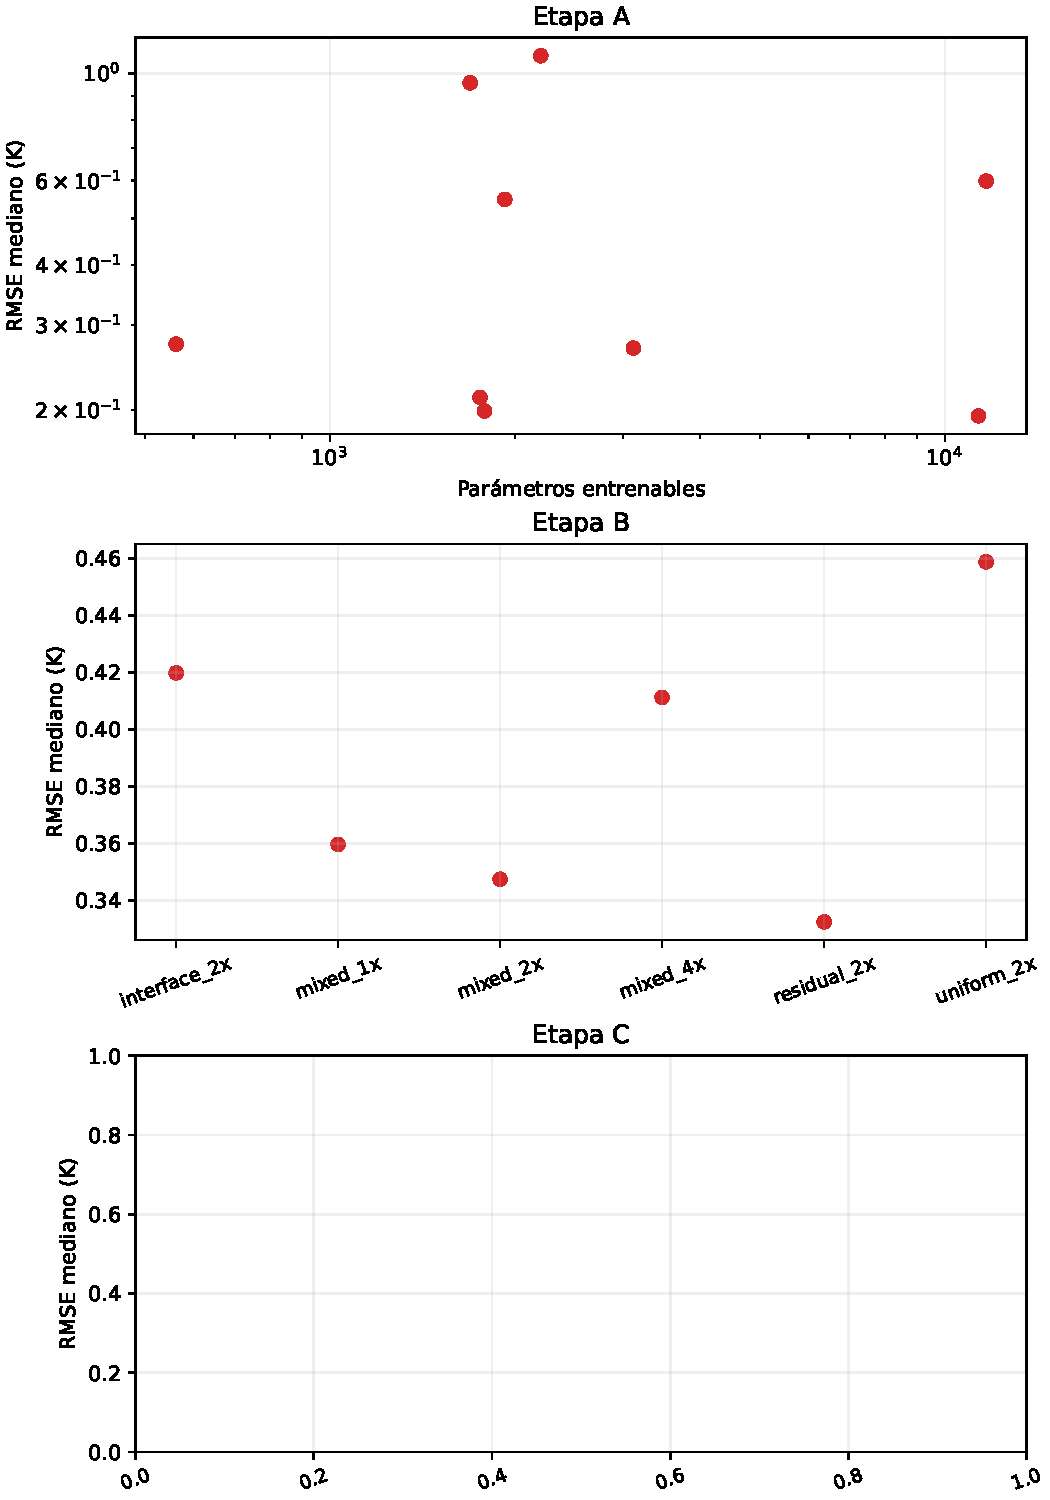
\includegraphics[width=.88\textwidth,height=.82\textheight,keepaspectratio]{explicit/selection.pdf}

\caption{Comparación de desarrollo. Verde: aceptación completa; rojo: al menos un rechazo. Los paneles corresponden a etapas distintas y no a un único factorial. Fuente: elaboración propia.}\end{figure}

\begin{figure}[htbp]\centering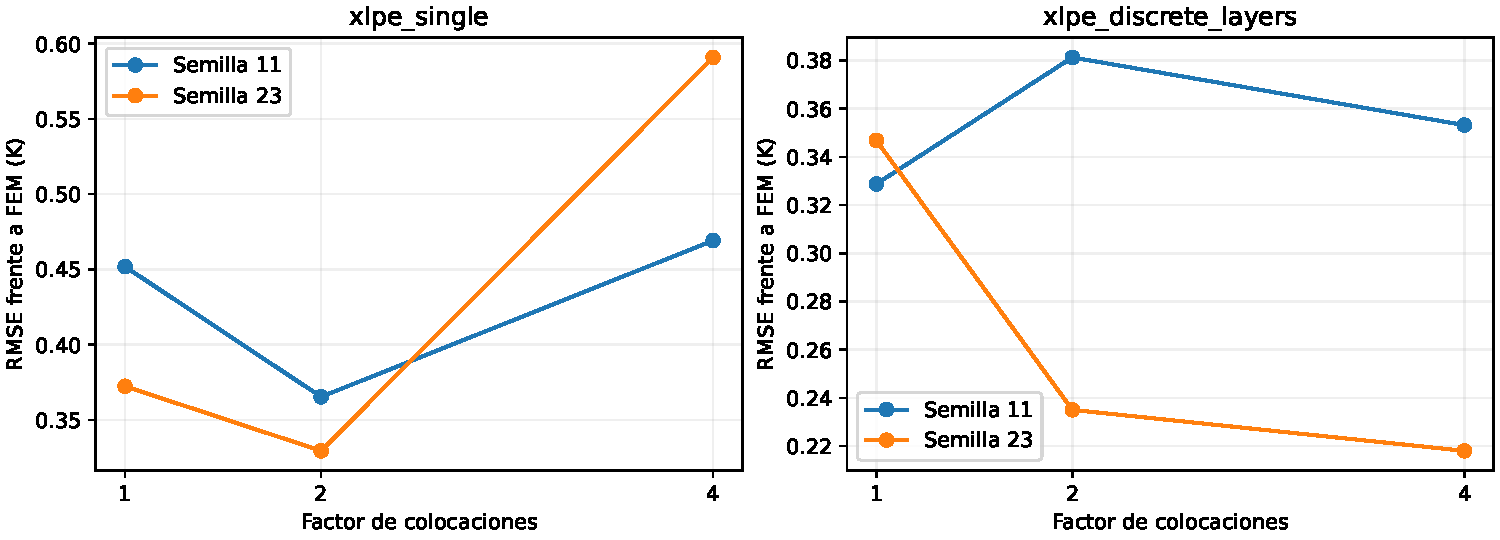
\includegraphics[width=\textwidth]{explicit/convergence.pdf}

\caption{Sensibilidad al número de colocaciones con la misma arquitectura y política geométrica. Fuente: elaboración propia.}\end{figure}

\begin{figure}[p]\centering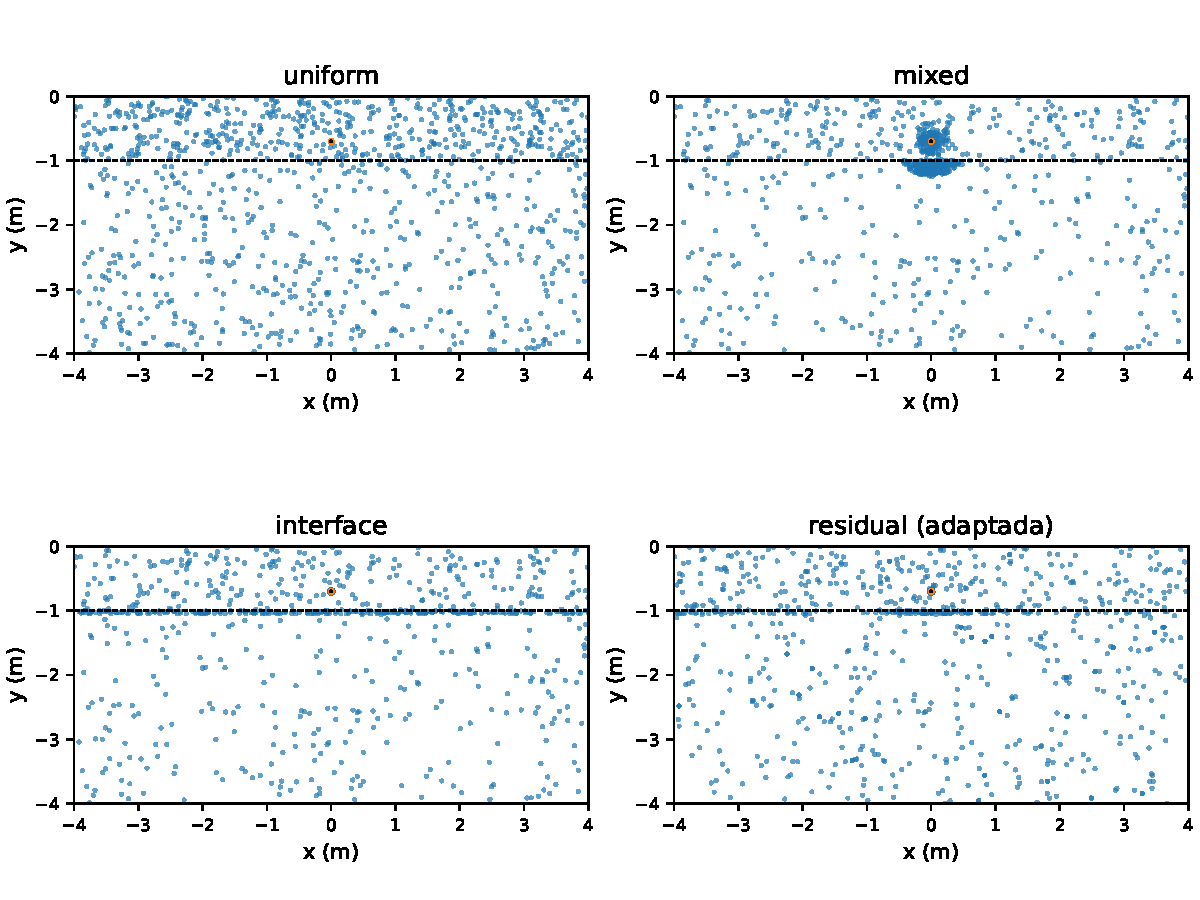
\includegraphics[width=\textwidth]{explicit/collocation_domain.pdf}

\caption{Cobertura del dominio para las cuatro políticas a igual presupuesto 2x, estratos y semilla 11. Azul: suelo; naranja: materiales del cable; líneas: interfaces geométricas. Se muestran colocaciones interiores, no las cuadraturas de trazas. Fuente: nubes archivadas; la política residual muestra la nube posterior a la adaptación.}\end{figure}

\begin{figure}[p]\centering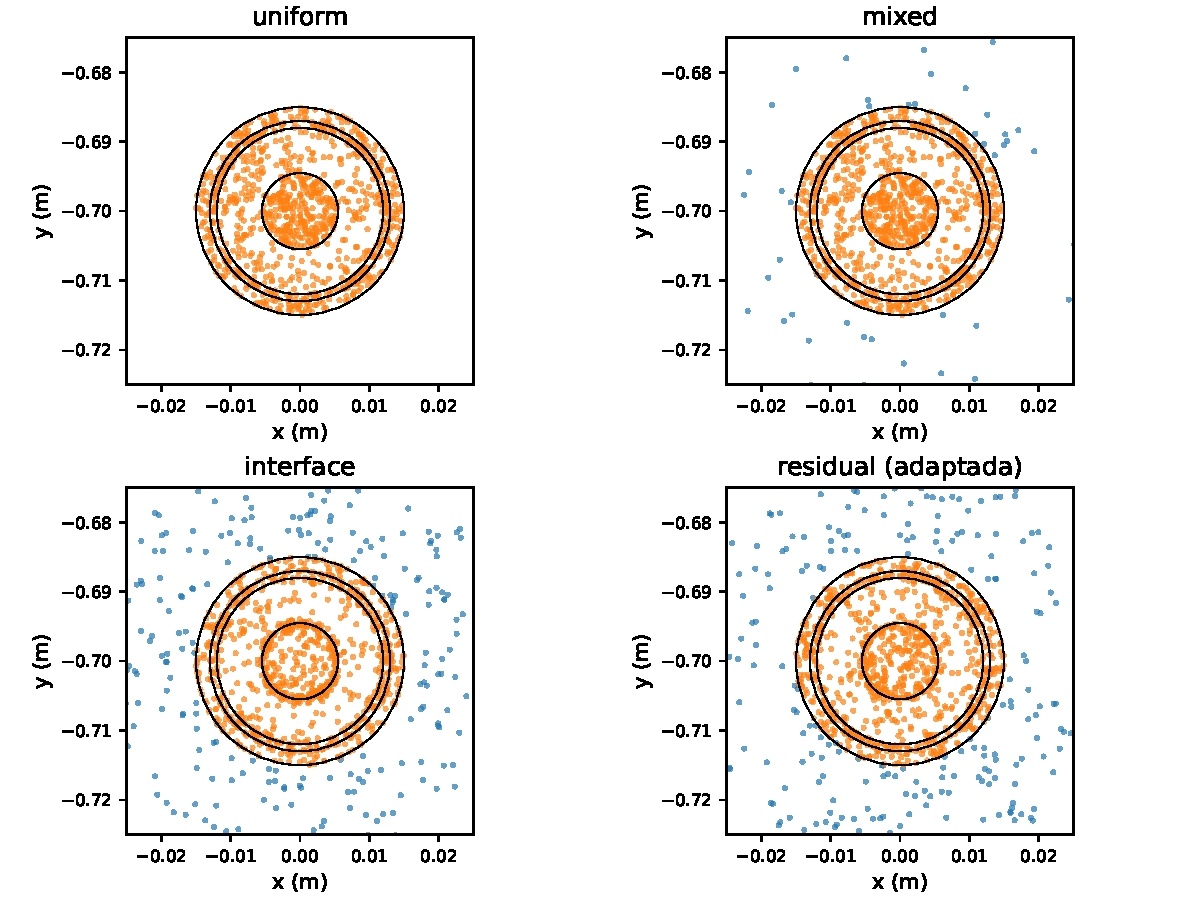
\includegraphics[width=\textwidth]{explicit/collocation_detail.pdf}

\caption{Detalle del cable para las cuatro políticas a igual presupuesto 2x, estratos y semilla 11. Azul: suelo; naranja: materiales del cable; líneas: interfaces geométricas. Se muestran colocaciones interiores, no las cuadraturas de trazas. Fuente: nubes archivadas; la política residual muestra la nube posterior a la adaptación.}\end{figure}


\subsection{EFECTO PIEL Y DISTRIBUCIÓN INTERIOR DEL CALOR}

El cálculo cilíndrico condicional, suponiendo R20 DC y conductor macizo homogéneo aislado, estima un incremento de pérdidas de 0,195--0,317\,\pct{} para el conductor XLPE pequeño y de 25,578--37,136\,\pct{} para los conductores grandes del catálogo, entre 90 y 20 °C. Estas cifras no certifican la resistencia AC de los cables publicados: construcción, frecuencia, temperatura y naturaleza del dato requieren procedencia primaria.

La comparación FEM 2D del caso Aras a igual potencia AC utilizó cuatro mallas por perfil de fuente. El cambio de Tmax al pasar de fuente uniforme a perfil piel fue $-0,004132$, $-0,004051$, $-0,004045$ y $-0,004045$ K. La malla fina tiene 380113 grados de libertad y balance de 0,002402\,\pct{}. La diferencia entre las dos últimas estimaciones del efecto es aproximadamente $4,1\times10^{-7}$ K. Se normalizó la fuente interpolada por su integral para impedir que un pequeño cambio de potencia contaminara la comparación de perfiles.

Este ensayo respalda que la redistribución radial resulta secundaria para la temperatura estacionaria de ese caso, frente al criterio de 0,1 K adoptado. No permite omitir el aumento de pérdidas AC ni extender la conclusión a proximidad, conductores segmentados o transitorios. La fuente no uniforme permanece disponible para todas las variantes y la conducción interior se resuelve siempre mediante la PDE.

\subsection{ACOPLAMIENTO LOCAL Y ALCANCE DE LA AMPACIDAD}

La formulación DC local se verificó en el caso coaxial con FEM y PINN explícitos: la referencia fina obtuvo 32,571582 °C y la PINN 32,575572 °C, diferencia de 0,003990 K. Este piloto demuestra la ejecución de la ley local de la Fórmula~\ref{for:fuente-dc-local}; no sustituye una campaña de confirmación de ampacidad. Las capacidades térmicas y las condiciones iniciales aún no se han utilizado para resolver una evolución temporal completa.

La verificación de corriente límite explícita está en ejecución. OE4 no se considera concluido con resultados de potencia fija.


\section{DISCUSIÓN E INTERPRETACIÓN}
\label{sec:discusion}

La pregunta principal es qué configuración satisface conjuntamente las ecuaciones, interfaces y referencia en el dominio ensayado. Una pérdida menor, un campo visualmente suave o una Tmax cercana no constituyen por sí solos aceptación. Los resultados negativos de redes pequeñas delimitan su utilidad con el presupuesto empleado, sin demostrar que una red mayor sea siempre preferible.

La selección secuencial permite estudiar decisiones concretas con un coste limitado, pero omite interacciones entre arquitectura, muestreo y entrenamiento. Una arquitectura descartada en A podría mejorar con otra distribución o presupuesto. Los resultados se interpretan como búsqueda preliminar controlada, no como optimización global ni clasificación universal de familias PINN. Las semillas pareadas reducen diferencias de diseño entre alternativas, pero dos o tres semillas no bastan para estimar colas de fallo poco frecuentes.

La referencia FEM también tiene error y depende de propiedades y contornos. Las pruebas de malla y el control analítico reducen incertidumbre numérica, sin validar una instalación. La incertidumbre de k, resistencia, contactos, pérdidas y humedad no se convierte en incertidumbre estadística mediante variación de semillas. Las inferencias sobre heterogeneidad se limitan a pares donde la diferencia física supera el cambio de discretización y la dispersión de los solucionadores aceptados.

El alcance temporal sigue siendo una extensión: disponer del operador $\rho c_pT_t$ no demuestra un solucionador transitorio verificado. La ampacidad normativa AC requiere pérdidas dieléctricas, pantallas, proximidad y condiciones de instalación que exceden los controles ejecutados. Las conclusiones de OE4 deben basarse en una búsqueda de corriente límite de la formulación explícita y no en tablas heredadas del modelo reducido.

\section{IMPACTO Y PRODUCTO REPRODUCIBLE}
\label{sec:impacto}

El impacto demostrado es metodológico y computacional: especificar una física común, detectar comparaciones incompatibles, seleccionar una receta con reglas previas, repetirla con semillas nuevas y conservar tanto aceptaciones como rechazos. El impacto profesional potencial consiste en identificar casos que merecen evaluación térmica detallada. No se afirman ahorros, incremento autorizado de capacidad ni superioridad temporal sobre FEM sin evidencia específica.

\chapter{CONCLUSIONES Y RECOMENDACIONES}
\label{ch:conclusiones}

Este capítulo debe cerrar la cadena entre problema, objetivos, resultados y contribución. Debido a que el plan no contiene evidencia final de construcción y evaluación, no se formulan conclusiones anticipadas. La estructura queda preparada para incorporar afirmaciones sustentadas después de completar el Capítulo~\ref{ch:propuesta-desarrollo}.

\section{CONCLUSIONES}

\pendiente{Redactar las conclusiones con base exclusiva en resultados verificados. Cada conclusión debe responder un objetivo, incluir la evidencia cuantitativa necesaria y declarar el dominio de validez.}

La versión final debe mantener el siguiente orden lógico:

\begin{enumerate}
  \item conclusión sobre el problema general y la utilidad demostrada del artefacto;
  \item conclusión sobre la especificación trazable y los requisitos del OE1;
  \item conclusión sobre la verificación, exactitud, consistencia física y robustez del OE2;
  \item conclusión sobre el efecto del contraste, patrón, extensión y proximidad en el OE3;
  \item conclusión sobre las discrepancias de ampacidad identificadas en el OE4;
  \item conclusión metodológica sobre los principios de diseño, la reproducibilidad y los límites del artefacto.
\end{enumerate}

Las conclusiones no deben repetir tablas ni presentar información nueva. Tampoco deben convertir una verificación computacional en validación de campo. Cuando un objetivo no se alcance, la conclusión debe explicar el resultado y su efecto sobre el alcance de la tesis.

\section{RECOMENDACIONES}

\pendiente{Formular recomendaciones después de cerrar las conclusiones. Cada recomendación debe derivarse de una limitación, un resultado o una condición observada durante la construcción y evaluación.}

Las recomendaciones podrán dirigirse a cuatro ámbitos, siempre que exista evidencia:

\begin{enumerate}
  \item uso del artefacto dentro del dominio verificado;
  \item mejoras de arquitectura, muestreo, pérdidas o tratamiento de interfaces;
  \item ampliación a régimen transitorio, humedad acoplada o validación experimental;
  \item prácticas de trazabilidad y verificación para futuros artefactos térmicos.
\end{enumerate}

No deben recomendarse decisiones sobre instalaciones reales, aumentos de capacidad ni sustitución de métodos normativos sin una validación independiente que supere el alcance declarado.



\clearpage
\begin{singlespace}
\printbibliography[heading=bibintoc,title={REFERENCIAS}]
\end{singlespace}

\setcounter{section}{0}
\renewcommand{\thesection}{\Alph{section}}
\renewcommand{\theHsection}{anexo.\arabic{section}}
\counterwithin{table}{section}
\renewcommand{\theHtable}{anexo.\arabic{section}.\arabic{table}}

\begin{landscape}
\chapter*{ANEXOS}
\addcontentsline{toc}{chapter}{ANEXOS}

\section{MATRIZ DE CONSISTENCIA}
\label{anx:matriz-consistencia}

La matriz conserva la relación entre problemas, objetivos, productos y evidencia. Se conservan HE1--HE4 como proposiciones contrastables del plan; los criterios determinan el estado de sus productos y no sustituyen las hipótesis por una declaración automática de cumplimiento.

\begin{table}[H]
\centering
\caption{Matriz de consistencia de la investigación. Fuente: Elaboración propia a partir del plan de tesis.}
\label{tab:matriz-consistencia}
\scriptsize
\setlength{\tabcolsep}{3pt}
\begin{tabularx}{\linewidth}{L{0.8cm}Y Y Y Y}
\toprule
\textbf{ID} & \textbf{Problema específico} & \textbf{Objetivo específico} & \textbf{Producto} & \textbf{Evidencia y criterio} \\
\midrule
1 & No existe una especificación formal que ordene cable, materiales, fuentes, contornos, interfaces y $\kx$. & Elaborar una especificación trazable de entradas, requisitos y criterios. & Especificación y matriz requisito--prueba. & Cobertura de requisitos, consistencia de unidades y trazabilidad. \\
2 & No se dispone de un paquete integrado de referencias para verificar el artefacto. & Construir y verificar el artefacto con referencias analíticas, manufacturadas, FEM y publicadas. & Artefacto versionado y expediente de aceptación. & Error de $\Tmax$, NRMSE, residuos, balance, convergencia y robustez. \\
3 & No se ha cuantificado de forma trazable el efecto de contraste, patrón, extensión y proximidad. & Aplicar el artefacto a escenarios controlados y consolidar la evidencia térmica. & Expediente de escenarios heterogéneos. & $T(x,y)$, $\Tmax$, $\Delta\Tmax$, punto caliente y cobertura. \\
4 & No se conocen las condiciones de mayor discrepancia entre representaciones heterogéneas y homogéneas. & Comparar la ampacidad de representaciones pareadas e identificar las mayores discrepancias. & Expediente comparativo de ampacidad. & $\Imax$, $\Delta I$, margen térmico, clasificación y límites. \\
\bottomrule
\end{tabularx}
\end{table}
\end{landscape}

Los productos corresponden a la especificación y los expedientes de la formulación explícita. La evidencia anterior de reconstrucción radial se conserva como antecedente. El cumplimiento de OE4 requiere una solución de corriente límite y su comparación FEM.

\section{MATRIZ DE OPERACIONALIZACIÓN}
\label{anx:operacionalizacion}

La operacionalización sigue una cadena de objetos. El producto de una etapa se convierte en parte de la entrada de la siguiente. Los parámetros físicos describen los casos y no se confunden con variables estadísticas de una población.

Se mantiene la cadena del plan: $\mathrm{VI1}=P_1$, $\mathrm{VI2}=\{\mathrm{VD1},R_2\}$, $\mathrm{VI3}=\{\mathrm{VD2},E_3\}$ y $\mathrm{VI4}=\{\mathrm{VD3},C_4\}$. Los objetos nuevos son el paquete físico $P_1$, las referencias $R_2$, los escenarios térmicos $E_3$ y los pares de representación $C_4$. Los indicadores numéricos están contenidos en los expedientes; no reemplazan esos objetos ni convierten las semillas en una población de instalaciones. Un producto restringido no se hereda como aceptación universal en la etapa siguiente.

\begin{table}[H]
\centering
\caption{Operacionalización por etapas del artefacto. Fuente: Elaboración propia.}
\label{tab:operacionalizacion}
\scriptsize
\setlength{\tabcolsep}{3pt}
\begin{tabularx}{\textwidth}{L{1.0cm}Y Y Y}
\toprule
\textbf{Etapa} & \textbf{Entrada} & \textbf{Salida} & \textbf{Indicadores} \\
\midrule
OE1 & Paquete de geometría, materiales, fuentes, contornos y requisitos. & Especificación trazable. & Cobertura, trazabilidad, unidades y supuestos. \\
OE2 & Especificación y referencias independientes. & Artefacto verificado y expediente de aceptación. & Error, NRMSE, residuos, balance, robustez y dominio. \\
OE3 & Artefacto aceptado y catálogo de escenarios. & Expediente de evidencia térmica. & $T(x,y)$, $\Tmax$, $\Delta\Tmax$, gradiente y punto caliente. \\
OE4 & Evidencia térmica y catálogo de pares. & Expediente comparativo de ampacidad. & $\Imax$, $\Delta I$, margen y clasificación del caso. \\
\bottomrule
\end{tabularx}
\end{table}

\section{MATRIZ REQUISITO--EVIDENCIA}

\begin{longtable}{L{1cm}L{4.5cm}L{8cm}}
\caption{Trazabilidad de requisitos críticos de la formulación explícita. Fuente: contrato físico, pruebas y expedientes de ejecución.}\label{tab:explicit-requirements}\\
\toprule ID & Requisito & Evidencia y límite \\
\midrule\endfirsthead
\toprule ID & Requisito & Evidencia y límite \\
\midrule\endhead
R1 & PDE en conductor, cada capa y suelo. & Pruebas parametrizadas de residuos y retropropagación de todas las variantes; campos FEM con etiquetas de cada material. La presencia de un residuo no acredita por sí sola aceptación numérica. \\
R2 & Continuidad de temperatura y flujo. & Pérdidas de transmisión y evaluación independiente de cada interfaz. En la red mixta se comprueban ambos flujos. Los fallos permanecen como rechazos. \\
R3 & Resolución de escalas milimétricas y métricas. & Coordenadas locales, presupuesto por material y pruebas de cobertura; comparación B a 1x, 2x y 4x con FEM. La admisibilidad se separa de la insensibilidad. \\
R4 & Fuente eléctrica trazable y no duplicada. & Contrato DC/AC, pruebas de integral de fuente piel y conservación de corriente DC con temperatura local; comparación FEM de perfiles a igual potencia. La procedencia eléctrica real sigue condicionada a fichas auténticas. \\
R5 & Referencia del mismo problema. & Identidad física, coordenadas comunes, SHA-256 del campo y puertas de refinamiento FEM. Las referencias reducidas no son intercambiables. \\
R6 & Elección sin seleccionar una semilla favorable. & Manifiestos A--C, configuración congelada y D con semillas 71, 83 y 97. Se publican todos los intentos. \\
R7 & Corriente límite con PDE interior. & Raíces FEM de tres mallas, corriente positiva aprendida y nueve intentos de confirmación. El error térmico aislado no sustituye las puertas completas. \\
R8 & Reproducción y documento consistente. & Fuentes y nubes archivadas, repetición A/B del mismo caso y semillas, pruebas automáticas, auditoría de referencias y construcción de tablas y PDF desde los registros. \\
\bottomrule
\end{longtable}

Las pruebas de operadores temporales verifican la forma matemática del término de almacenamiento y la exigencia de capacidad documentada. Una simulación transitoria completa no forma parte de la cobertura ejecutada.

\section{CASOS POR ETAPA Y COBERTURA}
\label{anx:catalogo-casos}

Los casos físicos están en \path{Benchmarks/explicit_study/cases/}. A utiliza coaxial angular y XLPE homogéneo. B y C utilizan XLPE homogéneo y estratos con salto exacto. D conserva esos dos casos para confirmación con semillas nuevas y añade relleno mejorado, zona seca cercana, zona seca lejana, Aras plano y Kim arena.

Los controles analíticos, manufacturados y de piel tienen otra finalidad y no se suman como réplicas de confirmación. La ampacidad DC añade un par heterogéneo--homogéneo con una regla explícita de promedio del suelo. Las geometrías publicadas se adaptan a contornos y fuentes controladas; sus temperaturas no se atribuyen al artefacto. El catálogo más amplio del plan incluye fuentes de propiedades y extensiones no ejecutadas, como humedad acoplada, k(T), datos estacionales y régimen transitorio. La presencia de un caso en archivos no demuestra cobertura experimental.

\section{REPRODUCCIÓN Y CONTRATO DE ARCHIVOS}
\label{anx:protocolo-reproduccion}

Los protocolos registrados son \path{docs/PROTOCOLO_EXPERIMENTAL_EXPLICITO.md} y \path{docs/PROTOCOLO_AMPACIDAD_EXPLICITA.md}, complementados por \path{docs/PROTOCOLO_CALIBRACION_INTERFACES.md}. La enmienda C2 responde a evidencia de B y precede a C y D. La copia congelada de la campaña y los manifiestos por etapa permiten reconstruir su secuencia. Los datos físicos se separan de anchura, profundidad, colocaciones, tasa, presupuesto y semillas. La identidad física incluye PDE, fuentes, interfaces y supuestos eléctricos; un campo reducido no puede sustituir una referencia explícita.

La secuencia comprende: ejecutar pruebas de operadores y muestreo; construir referencias FEM y pasar las puertas de malla; ejecutar A y elegir arquitectura; ejecutar B y analizar colocaciones; ejecutar C y C2 y congelar entrenamiento; ejecutar D con semillas independientes; resolver la extensión de corriente límite; generar tablas y figuras desde los JSON y compilar la tesis. Los comandos principales son \path{Benchmarks/full_study.py}, \path{Benchmarks/full_ampacity_study.py} y \path{Benchmarks/full_study_report.py}. El generador histórico no debe introducir nuevamente cifras reducidas en la tesis activa.

Los NPZ contienen coordenadas, regiones, pesos y temperaturas. Los expedientes PINN incluyen configuración, nubes iniciales y adaptadas, pesos entrenados, estados de optimización, fuentes e historial. Los estados FEM finales incluyen malla curva, etiquetas y grados de libertad. Los ensayos intermedios de la raíz de corriente conservan valores, balances y criterios; no se cuentan como problemas físicos adicionales.

Las semillas 11 y 23 y sus muestreos 101 y 103 pertenecen al desarrollo. Las semillas 71, 83 y 97 y sus muestreos 1001, 1003 y 1007 pertenecen a confirmación. El orquestador reutiliza solo resultados completos de la misma configuración. No se afirma reanudación exacta a mitad de L-BFGS: una ejecución interrumpida debe repetirse desde su configuración o disponer de un protocolo de restauración específico.

La PINN usa Python y PyTorch en Windows, precisión doble y un hilo por proceso; FEniCSx y Gmsh se ejecutan en Linux. Las versiones utilizadas se registran por corrida. Las reinstalaciones y repeticiones del modelo anterior no prueban una reinstalación limpia de este flujo. Las huellas permiten auditar procedencia sin inventar un commit para cambios de trabajo no confirmados en Git.

\section{EXPEDIENTE COMPLETO DE EJECUCIONES}
\label{anx:expediente-evidencia}

La tabla siguiente conserva las ejecuciones completas de A--D, incluidas las rechazadas. La misma información está en \path{Benchmarks/explicit_study/report/runs.csv}, con resúmenes de selección, convergencia y confirmación. El repositorio conserva el respaldo verificado de la tesis anterior; las tablas activas proceden de la formulación explícita.

\begingroup\footnotesize\setlength{\tabcolsep}{3pt}
\begin{longtable}{L{4cm}L{3.5cm}rrr}
\caption{Todas las ejecuciones de la campaña explícita. Fuente: manifiestos por etapa.}\label{tab:explicit-all}\\
\toprule
Etapa / configuración & Caso & Semilla & RMSE, K & Aceptada\\
\midrule\endfirsthead
\toprule
Etapa / configuración & Caso & Semilla & RMSE, K & Aceptada\\
\midrule\endhead
A/fourier\_w16\_d2 & coaxial\_angular & 11 & 0.507 & No\\
A/fourier\_w16\_d2 & coaxial\_angular & 23 & 0.306 & No\\
A/fourier\_w16\_d2 & xlpe\_single & 11 & 5.544 & No\\
A/fourier\_w16\_d2 & xlpe\_single & 23 & 1.672 & No\\
A/local\_w16\_d2 & coaxial\_angular & 11 & 8.475 & No\\
A/local\_w16\_d2 & coaxial\_angular & 23 & 0.244 & No\\
A/local\_w16\_d2 & xlpe\_single & 11 & 0.932 & No\\
A/local\_w16\_d2 & xlpe\_single & 23 & 0.982 & No\\
A/mixed\_w16\_d2 & coaxial\_angular & 11 & 0.146 & No\\
A/mixed\_w16\_d2 & coaxial\_angular & 23 & 0.185 & No\\
A/mixed\_w16\_d2 & xlpe\_single & 11 & 0.911 & No\\
A/mixed\_w16\_d2 & xlpe\_single & 23 & 0.939 & No\\
A/mixed\_w32\_d3 & coaxial\_angular & 11 & 0.302 & No\\
A/mixed\_w32\_d3 & coaxial\_angular & 23 & 0.242 & No\\
A/mixed\_w32\_d3 & xlpe\_single & 11 & 0.894 & No\\
A/mixed\_w32\_d3 & xlpe\_single & 23 & 1.125 & No\\
A/multipole\_w16\_d2 & coaxial\_angular & 11 & 0.069 & No\\
A/multipole\_w16\_d2 & coaxial\_angular & 23 & 0.023 & No\\
A/multipole\_w16\_d2 & xlpe\_single & 11 & 0.381 & No\\
A/multipole\_w16\_d2 & xlpe\_single & 23 & 0.329 & No\\
A/subdomain\_w16\_d2 & coaxial\_angular & 11 & 0.068 & No\\
A/subdomain\_w16\_d2 & coaxial\_angular & 23 & 0.019 & No\\
A/subdomain\_w16\_d2 & xlpe\_single & 11 & 0.357 & Sí\\
A/subdomain\_w16\_d2 & xlpe\_single & 23 & 0.406 & Sí\\
A/subdomain\_w16\_d3 & coaxial\_angular & 11 & 0.032 & No\\
A/subdomain\_w16\_d3 & coaxial\_angular & 23 & 0.059 & No\\
A/subdomain\_w16\_d3 & xlpe\_single & 11 & 0.744 & No\\
A/subdomain\_w16\_d3 & xlpe\_single & 23 & 0.479 & No\\
A/subdomain\_w32\_d3 & coaxial\_angular & 11 & 0.014 & Sí\\
A/subdomain\_w32\_d3 & coaxial\_angular & 23 & 0.017 & No\\
A/subdomain\_w32\_d3 & xlpe\_single & 11 & 0.452 & Sí\\
A/subdomain\_w32\_d3 & xlpe\_single & 23 & 0.372 & Sí\\
A/subdomain\_w8\_d2 & coaxial\_angular & 11 & 0.123 & No\\
A/subdomain\_w8\_d2 & coaxial\_angular & 23 & 0.067 & No\\
A/subdomain\_w8\_d2 & xlpe\_single & 11 & 0.426 & No\\
A/subdomain\_w8\_d2 & xlpe\_single & 23 & 0.820 & No\\
B/interface\_2x & xlpe\_discrete\_layers & 11 & 0.230 & No\\
B/interface\_2x & xlpe\_discrete\_layers & 23 & 0.545 & No\\
B/interface\_2x & xlpe\_single & 11 & 0.294 & Sí\\
B/interface\_2x & xlpe\_single & 23 & 0.618 & Sí\\
B/mixed\_1x & xlpe\_discrete\_layers & 11 & 0.329 & No\\
B/mixed\_1x & xlpe\_discrete\_layers & 23 & 0.347 & No\\
B/mixed\_1x & xlpe\_single & 11 & 0.452 & Sí\\
B/mixed\_1x & xlpe\_single & 23 & 0.372 & Sí\\
B/mixed\_2x & xlpe\_discrete\_layers & 11 & 0.381 & No\\
B/mixed\_2x & xlpe\_discrete\_layers & 23 & 0.235 & No\\
B/mixed\_2x & xlpe\_single & 11 & 0.365 & Sí\\
B/mixed\_2x & xlpe\_single & 23 & 0.329 & Sí\\
B/mixed\_4x & xlpe\_discrete\_layers & 11 & 0.353 & No\\
B/mixed\_4x & xlpe\_discrete\_layers & 23 & 0.218 & No\\
B/mixed\_4x & xlpe\_single & 11 & 0.469 & Sí\\
B/mixed\_4x & xlpe\_single & 23 & 0.591 & Sí\\
B/residual\_2x & xlpe\_discrete\_layers & 11 & 0.315 & No\\
B/residual\_2x & xlpe\_discrete\_layers & 23 & 0.350 & No\\
B/residual\_2x & xlpe\_single & 11 & 0.303 & Sí\\
B/residual\_2x & xlpe\_single & 23 & 0.372 & Sí\\
B/uniform\_2x & xlpe\_discrete\_layers & 11 & 0.490 & No\\
B/uniform\_2x & xlpe\_discrete\_layers & 23 & 0.428 & No\\
B/uniform\_2x & xlpe\_single & 11 & 0.627 & No\\
B/uniform\_2x & xlpe\_single & 23 & 0.249 & No\\
\bottomrule\end{longtable}\endgroup



\end{document}
